% =====================================================================
%  B.Tech Project report (draft)
%  Format: Times (TeX Gyre Termes), 12 pt, 1.5 line spacing.
%  Order: Title, Certificate, Contents, Lists, Abstract, Nomenclature,
%         Chapters, References, Appendix.
%  Items in red [[...]] are placeholders to be filled in.
% =====================================================================
\documentclass[12pt,a4paper,oneside]{report}
\usepackage[a4paper,left=3cm,right=2.5cm,top=2.5cm,bottom=2.5cm,headheight=15pt]{geometry}
\usepackage[T1]{fontenc}
\usepackage{newtxtext,newtxmath}
\usepackage{setspace}
\onehalfspacing
\usepackage{amsmath,bm}
\usepackage{booktabs,array,tabularx,longtable,multirow}
\usepackage{graphicx}
\usepackage[dvipsnames]{xcolor}
\usepackage{tikz}
\usetikzlibrary{arrows.meta,calc,patterns,decorations.pathreplacing}
\usepackage{caption,subcaption}
\usepackage{float}
\usepackage{fancyhdr}
\usepackage{enumitem}
\usepackage{siunitx}
\usepackage{microtype}
\usepackage{titlesec}
\usepackage[nottoc]{tocbibind}
\usepackage[colorlinks=true,linkcolor=black,citecolor=black,urlcolor=black]{hyperref}

\sisetup{per-mode=symbol,detect-all}
\def\UrlBreaks{\do\/\do\_\do\.}
\captionsetup{font=small,labelfont=bf,labelsep=period}
\numberwithin{equation}{chapter}
\numberwithin{figure}{chapter}
\numberwithin{table}{chapter}
\graphicspath{{figures/}{../figures/}}
\setlist{itemsep=2pt,topsep=4pt}

\titleformat{\chapter}[display]{\normalfont\bfseries\centering}{\large CHAPTER \thechapter}{6pt}{\Large\MakeUppercase}
\titlespacing*{\chapter}{0pt}{0pt}{24pt}
\titleformat{\section}{\normalfont\large\bfseries}{\thesection}{0.8em}{}
\titleformat{\subsection}{\normalfont\normalsize\bfseries}{\thesubsection}{0.8em}{}

\pagestyle{fancy}
\fancyhf{}
\fancyfoot[C]{\thepage}
\renewcommand{\headrulewidth}{0pt}
\fancypagestyle{plain}{\fancyhf{}\fancyfoot[C]{\thepage}\renewcommand{\headrulewidth}{0pt}}

\definecolor{corr}{HTML}{C0392B}
\definecolor{note}{HTML}{1F4E79}
\newcommand{\fillin}[1]{\textcolor{red}{[[#1]]}}
\newcommand{\Izz}{I_{zz}}
\newcommand{\rp}{r_p}
\newcommand{\tmin}{t_{\min}}
\newcommand{\tmax}{t_{\max}}

\begin{document}

% =====================================================================
%  TITLE PAGE
% =====================================================================
\begin{titlepage}
\centering
\vspace*{0.5cm}
{\Large\bfseries MODELLING AND ANALYSIS OF\\[4pt] SOFT BENDING ACTUATOR\par}
\vspace{1.9cm}
{\normalsize A report submitted in partial fulfilment of the requirements\\ for the award of the degree of\par}
\vspace{0.4cm}
{\large\bfseries Bachelor of Technology\par}
\vspace{0.2cm}
{\normalsize in\par}
\vspace{0.2cm}
{\large Mechanical Engineering\par}
\vspace{1.0cm}
{\normalsize by\par}
\vspace{0.3cm}
{\large\bfseries Rudranarayan Pradhan\par}
{\normalsize Roll No.\ 23ME31022\par}
\vspace{0.9cm}
{\normalsize Under the supervision of\par}
\vspace{0.3cm}
{\large Prof.\ Vikranth Rachrela\par}
\vfill
\IfFileExists{figures/iitkgp_logo.png}{
\includegraphics[height=3.2cm]{iitkgp_logo.png}\par}{{\normalsize \fillin{IIT Kharagpur logo}\par}}
\vspace{0.5cm}
{\large Department of Mechanical Engineering\\ Indian Institute of Technology Kharagpur\par}
\vspace{0.3cm}
{\normalsize November 2026\par}
\end{titlepage}

\pagenumbering{roman}
\setcounter{page}{2}

% =====================================================================
%  DECLARATION
% =====================================================================
\chapter*{Declaration}
\addcontentsline{toc}{chapter}{Declaration}
I certify that
\begin{enumerate}[label=(\alph*)]
\item the work contained in this report is original and has been done by me under the guidance of my
supervisor;
\item the work has not been submitted to any other institute for any degree or diploma;
\item I have followed the guidelines provided by the Institute in preparing the report;
\item I have conformed to the norms and guidelines given in the Ethical Code of Conduct of the Institute;
\item whenever I have used materials (data, theoretical analysis, figures and text) from other sources, I
have given due credit to them by citing them in the text of the report and giving their details in the
references.
\end{enumerate}

\vspace{2.5cm}
\noindent
\begin{tabular}{@{}l}
\rule{6cm}{0.4pt}\\
Rudranarayan Pradhan\\
Roll No.\ 23ME31022\\
Date: \rule{3cm}{0.4pt}\\
Place: \rule{3cm}{0.4pt}
\end{tabular}

% =====================================================================
%  CERTIFICATE
% =====================================================================
\chapter*{Certificate}
\addcontentsline{toc}{chapter}{Certificate}
This is to certify that the report entitled \textbf{``Modelling and Analysis of Soft Bending Actuator''}, submitted by \textbf{Rudranarayan Pradhan} (Roll No.\ 23ME31022) to the Indian Institute of
Technology Kharagpur in partial fulfilment of the requirements for the award of the degree of Bachelor of
Technology in Mechanical Engineering, is a record of the work carried out by the candidate under my
supervision during the seventh semester (Autumn Semester, 2026--27).

\vspace{2.5cm}
\noindent
\begin{tabular}{@{}l}
\rule{6cm}{0.4pt}\\
Prof.\ Vikranth Rachrela\\
Professor\\
Department of Mechanical Engineering\\
Indian Institute of Technology Kharagpur\\
Date: \rule{3cm}{0.4pt}\\
Place: \rule{3cm}{0.4pt}
\end{tabular}

% =====================================================================
%  CONTENTS AND LISTS
% =====================================================================
\tableofcontents
\listoffigures
\listoftables

% =====================================================================
%  ABSTRACT
% =====================================================================
\chapter*{Abstract}
\addcontentsline{toc}{chapter}{Abstract}
A soft pneumatic bending actuator is studied in which a silicone cylinder carries an off-centre
(eccentric) cavity. When the cavity is pressurised the cylinder bends toward its thicker wall. The aim of
the work is the relation between the cavity pressure and the bending of the actuator.

The cross-section properties, the eccentric thrust moment and the Euler--Bernoulli bending response are
derived in closed form. A free-body argument shows that the thrust moment is uniform along the actuator
for any material law. An equilibrium argument for the in-plane wall stresses then shows that, for a
bare (unreinforced) actuator, linear elasticity multiplies the beam curvature by $(1-2\nu)$, which
vanishes for nearly incompressible silicone. The bending that a bare actuator does show is therefore a
finite-strain effect: the thin wall lengthens more than the thick wall, at second order in its hoop
strain, and the response ends at a ballooning limit pressure.

These results were checked with nonlinear three-dimensional finite-element (FE) models built in COMSOL
Multiphysics 6.4: hyperelastic (neo-Hookean) silicone with a nearly incompressible mixed formulation, a
follower pressure on every face of the cavity, and an optional inextensible hoop sleeve modelled as a
weak-form surface energy. For a placeholder design ($R=10$, $r=4$, $r_p=\SI{3}{mm}$, $l=\SI{100}{mm}$,
$E=\SI{0.6}{MPa}$) the tip angle of the sleeved actuator agrees with the beam formula within 1\,\% at
$P/E=0.017$ and within 5\,\% at $P/E=0.033$, and exceeds it at higher pressure. The bare actuator bends only
11\,\% of the beam prediction at $P/E=0.017$, and its response steepens strongly with pressure, as the
analysis predicts.

A tapered actuator with four chambers, intended to bend in any direction, was then modelled in COMSOL
with the real cavity pressure and nearly incompressible silicone. With an assumed modulus $E=\SI{0.07}{MPa}$, the
bare four-chamber actuator balloons at \SI{11.7}{kPa} ($P/\mu=0.50$), while the sleeved actuator bends
smoothly to \ang{47} at \SI{10}{kPa} and \ang{95} at \SI{15}{kPa}. Beyond about \SI{15}{kPa} the computed
local stress and element distortion grow rapidly; whether this is physical or numerical is not yet
resolved, so larger bending angles, contact and grasping forces are left for future work. All geometry and
material values are placeholders; no experiment has been carried out yet.

\vspace{0.5em}
\noindent\textbf{Keywords:} soft robotics, pneumatic actuator, hyperelasticity, ballooning, finite-element
analysis, fibre reinforcement.

% =====================================================================
%  NOMENCLATURE
% =====================================================================
\chapter*{Nomenclature}
\addcontentsline{toc}{chapter}{Nomenclature}
\begin{longtable}{@{}p{2.4cm}p{9.8cm}l@{}}
\toprule
Symbol & Meaning & Unit\\
\midrule
\endhead
$R$ & outer radius of the actuator & mm\\
$r$ & cavity radius (single-cavity actuator) & mm\\
$\rp$ & cavity eccentricity (offset of the cavity centre from the axis) & mm\\
$l$, $L$ & pressurised length; total length of the four-chamber actuator & mm\\
$\tmin$, $\tmax$ & thinnest and thickest wall, $R\mp\rp-r$ & mm\\
$t(\phi)$ & wall thickness along a ray at angle $\phi$ from the thin side & mm\\
$A$, $A_c$ & elastomer area of the section; cavity area & mm$^2$\\
$\bar y$ & position of the neutral axis & mm\\
$\Izz$ & second moment of area about the neutral axis & mm$^4$\\
$e$ & moment arm of the thrust about the neutral axis & mm\\
$P$ & gauge pressure in the cavity & kPa\\
$F$, $M$ & axial thrust on the tip cap; bending moment & N, N\,mm\\
$\kappa$, $\rho$ & curvature; radius of curvature & mm$^{-1}$, mm\\
$\theta$, $\delta$ & tip angle (tip rotation); transverse tip deflection & deg, mm\\
$E$, $\mu$, $\nu$ & small-strain Young's modulus, shear modulus, Poisson's ratio & MPa, MPa, --\\
$\kappa_b$ & bulk modulus & MPa\\
$C_{10},C_{20},C_{30}$ & Yeoh coefficients (neo-Hookean: $C_{10}=\mu/2$, others zero) & MPa\\
$\lambda$, $\lambda_h$ & stretch; hoop stretch & --\\
$J$ & local volume ratio $\det\bm F$ & --\\
$\bm F$ & deformation gradient & --\\
$k_s$ & hoop-sleeve stiffness (penalty) & N/mm\\
$e_h$ & Green strain of the outer surface in the hoop direction & --\\
$W$ & strain-energy density & MPa\\
$\bar I_1$ & first invariant of the isochoric right Cauchy--Green tensor & --\\
$\varepsilon_0$, $\varepsilon_x$ & centroidal axial strain; axial strain & --\\
$\sigma_x$, $\sigma_y$, $\sigma_z$ & normal stresses & MPa\\
$\alpha$ & half-angle of a chamber sector (four-chamber actuator) & deg\\
$a(x)$, $b(x)$ & inner and outer radius of a chamber at position $x$ & mm\\
\midrule
FE & finite element(s) & \\
NA & neutral axis & \\
\bottomrule
\end{longtable}

\clearpage
\pagenumbering{arabic}

% =====================================================================
\chapter{Introduction}\label{ch:intro}
% =====================================================================

\section{Background}
Soft robots built from elastomers can bend, grip and conform to objects without rigid joints, which makes
them attractive for handling delicate or irregular objects and for medical devices. Among their actuators,
fluid-driven elastomer actuators are the most common: a cavity in the elastomer is pressurised with air or
liquid and the body deforms \cite{gorissen2017,marchese2015}. How a given pressure turns into a given
motion depends on the geometry, on the strongly nonlinear behaviour of the elastomer and on any
reinforcement such as fibres or inextensible layers \cite{polygerinos2015,connolly2017}. A model of this
relation is needed both to design the actuator and to control it.

\section{The actuator studied}
The actuator considered first is a solid silicone cylinder of outer radius $R$ and pressurised length $l$,
with a circular cavity of radius $r$ whose centre is offset by $\rp$ from the axis (Figure~\ref{fig:geometry}).
One wall is therefore thin, $\tmin=R-\rp-r$, and the opposite wall thick, $\tmax=R+\rp-r$. The base is clamped,
the far end is closed by a solid cap, and the cavity is pressurised to a gauge pressure $P$. The actuator
bends toward the thick wall. The study is later extended to a tapered actuator with four chambers, which can
bend in any direction by pressurising one chamber or a combination of chambers.

\begin{figure}[H]
\centering
\begin{subfigure}[b]{0.52\textwidth}\centering
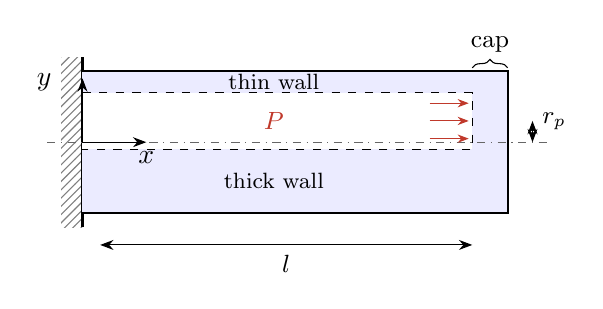
\begin{tikzpicture}[scale=0.9]
  \fill[pattern=north east lines,pattern color=black!50] (-0.3,-1.2) rectangle (0,1.2);
  \draw[thick] (0,-1.2) -- (0,1.2);
  \fill[blue!8] (0,-1) rectangle (6,1);
  \draw[thick] (0,1) -- (6,1) -- (6,-1) -- (0,-1);
  \fill[white] (0,-0.1) rectangle (5.5,0.7);
  \draw[dashed] (0,0.7) -- (5.5,0.7) -- (5.5,-0.1) -- (0,-0.1);
  \draw[dash dot,black!60] (-0.5,0) -- (6.6,0);
  \draw[-{Stealth}] (0,0) -- (0.9,0) node[below] {$x$};
  \draw[-{Stealth}] (0,0) -- (0,0.9);
  \node[left] at (-0.3,0.85) {$y$};
  \draw[{Stealth}-{Stealth}] (6.35,0) -- (6.35,0.3) node[right,font=\small] {$\rp$};
  \draw[{Stealth}-{Stealth}] (0.25,-1.45) -- (5.5,-1.45) node[midway,below,font=\small] {$l$};
  \draw[decorate,decoration={brace,amplitude=3pt}] (5.5,1.05) -- (6,1.05) node[midway,above=2pt,font=\small] {cap};
  \foreach \y in {0.05,0.3,0.55} \draw[-{Stealth[length=4pt]},corr] (4.9,\y) -- (5.45,\y);
  \node[corr,font=\small] at (2.7,0.3) {$P$};
  \node[font=\footnotesize] at (2.7,0.85) {thin wall};
  \node[font=\footnotesize] at (2.7,-0.55) {thick wall};
\end{tikzpicture}
\caption{Side view (bending plane $x$--$y$).}
\end{subfigure}\hfill
\begin{subfigure}[b]{0.44\textwidth}\centering
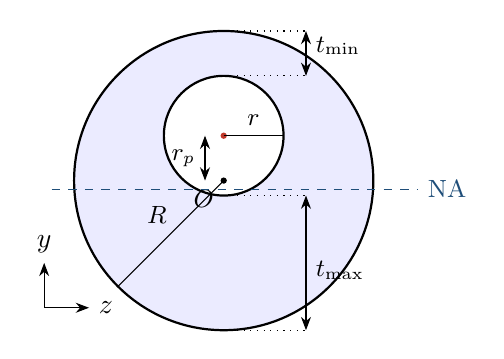
\begin{tikzpicture}[scale=0.95]
  \fill[blue!8] (0,0) circle (2);
  \draw[thick] (0,0) circle (2);
  \fill[white] (0,0.6) circle (0.8);
  \draw[thick] (0,0.6) circle (0.8);
  \draw[-{Stealth}] (-2.4,-1.7) -- (-1.8,-1.7) node[right] {$z$};
  \draw[-{Stealth}] (-2.4,-1.7) -- (-2.4,-1.1) node[above] {$y$};
  \fill (0,0) circle (1.2pt) node[below left,font=\small] {$O$};
  \fill[corr] (0,0.6) circle (1.2pt);
  \draw (0,0.6) -- (0.8,0.6) node[midway,above,font=\small] {$r$};
  \draw (0,0) -- (-1.414,-1.414) node[midway,above left,font=\small,xshift=2pt] {$R$};
  \draw[{Stealth}-{Stealth}] (-0.25,0) -- (-0.25,0.6) node[midway,left,font=\small] {$\rp$};
  \draw[dashed,note] (-2.3,-0.114) -- (2.6,-0.114) node[right,font=\small] {NA};
  \draw[{Stealth}-{Stealth}] (1.1,1.4) -- (1.1,2.0);
  \node[right,font=\small] at (1.1,1.8) {$\tmin$};
  \draw[{Stealth}-{Stealth}] (1.1,-0.2) -- (1.1,-2.0);
  \node[right,font=\small] at (1.1,-1.2) {$\tmax$};
  \draw[dotted] (0,1.4) -- (1.15,1.4); \draw[dotted] (0,-0.2) -- (1.15,-0.2);
  \draw[dotted] (0,2.0) -- (1.15,2.0); \draw[dotted] (0,-2.0) -- (1.15,-2.0);
\end{tikzpicture}
\caption{Cross-section.}
\end{subfigure}
\caption[Eccentric-cavity actuator: geometry and coordinate frame]{Eccentric-cavity actuator: geometry and coordinate frame. The origin $O$ is the centre of the outer
circle, the cavity centre is at $(y,z)=(\rp,0)$ and the neutral axis (NA) lies at $y=\bar y<0$. Not to scale.}
\label{fig:geometry}
\end{figure}

\section{Objectives}
\begin{enumerate}
\item Derive the pressure-to-bending relation of the eccentric-cavity actuator in closed form and state the
assumptions under which it holds.
\item Build nonlinear three-dimensional FE models in COMSOL Multiphysics that do not rely on those
assumptions, and use them to test the closed-form result for a bare and for a fibre-reinforced actuator.
\item Extend the model to a tapered four-chamber actuator for multi-directional bending and find how far
it can bend under real pressure.
\end{enumerate}

\section{Scope and limitations}
This report covers modelling only. The geometry and material values used are \emph{placeholders} chosen to
make the models concrete; the real design, the silicone and its measured constants are still to be fixed,
and no experiment has been carried out. The silicone is modelled as neo-Hookean. Gravity, viscoelasticity
and the Mullins effect are not modelled. Contact with objects, and hence grasping forces, are not part of
the results reported here (Section~\ref{sec:grasp}).

\section{Organisation of the report}
Chapter~\ref{ch:theory} derives the analytical model. Chapter~\ref{ch:method} describes how the FE models were
built, loaded, meshed and solved in COMSOL. Chapter~\ref{ch:results} presents the results for the
single-cavity actuator and for the four-chamber actuator. Chapter~\ref{ch:discussion} discusses what the
results mean and what limits them, and Chapter~\ref{ch:conclusion} gives the conclusions and the planned
next steps.

% =====================================================================
\chapter{Analytical Model}\label{ch:theory}
% =====================================================================
Units throughout: \si{mm}, \si{N}, \si{MPa} ($\SI{1}{MPa}=\SI{1000}{kPa}=\SI{1}{N/mm^2}$).
Axes: $x$ along the actuator (base at $x=0$); $y$ in the section from the outer centre toward the cavity
centre; $z$ completes the right-handed frame. Bending is about $z$, toward $-y$.

\section{Assumptions}
\begin{enumerate}[label=(A\arabic*)]
\item The material is isotropic, homogeneous, rate-independent and (nearly) incompressible.
\item The pressure is uniform in the cavity; gravity and external loads are neglected; the base is clamped
and the tip is free.
\item \emph{Beam model only:} plane sections remain plane, the cross-section keeps its shape, and every
longitudinal fibre is in uniaxial stress.
\end{enumerate}
Assumption (A3) holds when a hoop reinforcement carries the circumferential load. Section~\ref{sec:poisson}
shows that it fails for a bare actuator.

\section{Cross-section properties}\label{sec:section}
The section properties follow from the composite-area method and the parallel-axis theorem
\cite{gere2013}. The elastomer area is the outer disc minus the cavity:
\begin{equation}
A = \pi\,(R^2-r^2). \label{eq:A}
\end{equation}
Treating the cavity as a negative area centred at $y=\rp$, the neutral axis lies at
\begin{equation}
\bar y = \frac{\pi R^2\cdot 0 - \pi r^2\rp}{\pi R^2-\pi r^2} = -\,\frac{r^2\,\rp}{R^2-r^2}, \label{eq:ybar}
\end{equation}
on the thick-wall side of the outer centre. By the parallel-axis theorem applied to each disc,
\begin{equation}
\Izz = \Big[\frac{\pi R^4}{4} + \pi R^2\bar y^{\,2}\Big] - \Big[\frac{\pi r^4}{4} + \pi r^2(\rp-\bar y)^2\Big].
\end{equation}
With $\rp-\bar y = R^2\rp/(R^2-r^2)$ the two shift terms combine to $-\pi R^2r^2\rp^2/(R^2-r^2)$, so
\begin{equation}
\Izz = \frac{\pi\,(R^4-r^4)}{4} - \frac{\pi R^2 r^2 \rp^2}{R^2-r^2}. \label{eq:I}
\end{equation}
The first term is the concentric hollow cylinder; the second is the stiffness lost by moving the hole
off-centre.

\section{Pressure loading}\label{sec:load}
The pressure acts on the inside face of the tip cap, whose projected area is the cavity
area,\footnote{The resultant of a uniform pressure on a surface, in a given direction, equals the pressure
times the area of the surface projected on a plane normal to that direction; for the flat inner face of the
cap this is simply the cavity area $\pi r^2$. The same argument gives the axial load in a closed thin-walled
pressure vessel \cite{gere2013}.} giving the thrust
\begin{equation}
F = P\,A_c = P\,\pi r^2 . \label{eq:F}
\end{equation}
Its resultant passes through the cavity centre $y=\rp$, at a distance
\begin{equation}
e = \rp - \bar y = \frac{R^2\,\rp}{R^2-r^2} \label{eq:e}
\end{equation}
from the neutral axis, so the bending moment is
\begin{equation}
M = F\,e = \frac{\pi P R^2 r^2 \rp}{R^2-r^2}. \label{eq:M}
\end{equation}

\begin{figure}[H]
\centering
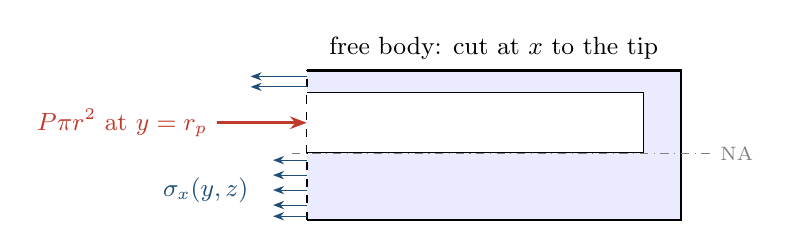
\begin{tikzpicture}[scale=0.95]
  \fill[blue!8] (0,-1) rectangle (5,1);
  \draw[thick] (0,1) -- (5,1) -- (5,-1) -- (0,-1);
  \draw[thick,dashed] (0,-1) -- (0,1);
  \fill[white] (0,-0.1) rectangle (4.5,0.7);
  \draw (0,0.7) -- (4.5,0.7) -- (4.5,-0.1) -- (0,-0.1);
  \node[font=\small] at (2.5,1.3) {free body: cut at $x$ to the tip};
  \draw[-{Stealth[length=6pt]},very thick,corr] (-1.2,0.3) -- (0,0.3);
  \node[corr,left,font=\small] at (-1.2,0.3) {$P\pi r^2$ at $y=\rp$};
  \foreach \y in {0.78,0.92} \draw[-{Stealth[length=4pt]},note] (0,\y) -- (-0.75,\y);
  \foreach \y in {-0.2,-0.4,-0.6,-0.8,-0.95} \draw[-{Stealth[length=4pt]},note] (0,\y) -- (-0.45,\y);
  \node[note,font=\small] at (-1.35,-0.6) {$\sigma_x(y,z)$};
  \draw[dash dot,black!50] (-0.2,-0.114) -- (5.4,-0.114) node[right,font=\scriptsize] {NA};
\end{tikzpicture}
\caption[Free body from a cut to the tip]{Free body from a cut at $x$ to the tip, silicone together with the enclosed fluid.}
\label{fig:fbd}
\end{figure}

\paragraph{The moment is uniform along the length.} Cut the actuator at any $x$ and take the free body from
the cut to the tip \emph{including the fluid it encloses} (Figure~\ref{fig:fbd}). No external force acts on
it except at the cut, so
\begin{equation}
\int_A \sigma_x\,dA = P\pi r^2 ,\qquad \int_A \sigma_x\,(y-\rp)\,dA = 0 . \label{eq:fbd}
\end{equation}
The wall is in net tension $N=P\pi r^2$ acting through the cavity centre, which about the neutral axis is
the moment $M=Ne$ of eq.~(\ref{eq:M}), at every $x$ and for any material law.\footnote{This free-body
argument uses statics only and is derived here for the eccentric cavity. The same balance, between the
moment of the pressure on the distal cap and the moment of the elastomer stresses, is the basis of the
quasi-static model of fibre-reinforced bending actuators in \cite{polygerinos2015}.} Equation~(\ref{eq:fbd}) fixes
only the \emph{resultants} of $\sigma_x$; relating them to strain needs a constitutive assumption.

\section{Euler--Bernoulli response}\label{sec:beam}
Under (A3), $\sigma_x = E\varepsilon_x$ with $\varepsilon_x=\varepsilon_0+\kappa(y-\bar y)$, and the
Euler--Bernoulli moment--curvature relation \cite{gere2013,timoshenko1970} gives
\begin{equation}
\kappa = \frac{M}{E\Izz} = \frac{\pi P R^2 r^2 \rp}{E\,\Izz\,(R^2-r^2)}. \label{eq:kappa}
\end{equation}
Here $E$ is the small-strain modulus, $E=3\mu=6C_{10}$ for an incompressible
solid.\footnote{For an isotropic linear-elastic solid $E=2\mu(1+\nu)$, so $E=3\mu$ when $\nu=1/2$
\cite{timoshenko1970}. For the neo-Hookean and Yeoh models the small-strain shear modulus is $\mu=2C_{10}$
\cite{treloar1975,holzapfel2000,yeoh1993}.} Since $M$ is uniform,
the centreline is a circular arc and the tip angle is
\begin{equation}
\theta = \kappa\,l = \frac{\pi P R^2 r^2 \rp\, l}{E\,\Izz\,(R^2-r^2)}, \label{eq:theta}
\end{equation}
linear in $P$. The transverse tip deflection of an arc of radius $\rho=1/\kappa$ (constant-curvature
geometry \cite{webster2010}) is
\begin{equation}
\delta = \frac{1-\cos\theta}{\kappa} \;\approx\; \frac{\theta\, l}{2}\quad(\theta\ll1). \label{eq:delta}
\end{equation}
In non-dimensional form, with $\hat I=\Izz/R^4$,
\begin{equation}
\theta = \frac{P}{E}\,\frac{l}{R}\,f\!\left(\frac{r}{R},\frac{\rp}{R}\right),\qquad
f = \frac{\pi (r/R)^2(\rp/R)}{\hat I\,\big(1-(r/R)^2\big)} . \label{eq:nondim}
\end{equation}

\begin{table}[H]
\centering\small
\caption[Beam model for the placeholder design]{Beam model for the placeholder design $R=10$, $r=4$, $\rp=3$, $l=\SI{100}{mm}$, $E=\SI{0.6}{MPa}$.}
\label{tab:example}
\begin{tabular}{@{}lr@{\qquad}lr@{}}
\toprule
\multicolumn{2}{c}{Section, eqs.~(\ref{eq:A})--(\ref{eq:e})} & \multicolumn{2}{c}{Response at $P=\SI{20}{kPa}$}\\
\midrule
$A$ & \SI{263.9}{mm^2} & $F$ & \SI{1.005}{N}\\
$\bar y$ & \SI{-0.571}{mm} & $M$ & \SI{3.590}{N\,mm}\\
$\Izz$ & \SI{7114.4}{mm^4} & $\kappa$ & \SI{8.41e-4}{mm^{-1}}\\
$e$ & \SI{3.571}{mm} & $\theta$ & \ang{4.82}\\
$\tmin,\ \tmax$ & \SI{3}{mm}, \SI{9}{mm} & $\delta$ (arc / small angle) & \SI{4.203}{mm} / \SI{4.206}{mm}\\
$\hat I$, $f$ & 0.7114, 0.2523 & & \\
\bottomrule
\end{tabular}
\end{table}

\section{The bare actuator: effect of the in-plane wall stresses}\label{sec:poisson}
The pressure also loads the wall \emph{in the plane of the section}: radial compression at the cavity
surface and hoop tension around it. Assumption (A3) ignores these stresses. In linear isotropic elasticity
they enter the axial strain through Poisson's ratio (generalised Hooke's law \cite{timoshenko1970}),
\begin{equation}
\sigma_x = E\big[\varepsilon_0 + \kappa(y-\bar y)\big] + \nu\,(\sigma_y+\sigma_z). \label{eq:hooke}
\end{equation}
The in-plane stresses need not be solved: away from the ends they satisfy
$\partial_\beta\sigma_{\alpha\beta}=0$ with a traction-free outer boundary and the traction $P\bm m$ on the
cavity boundary. Using the identities
$\partial_\beta(\sigma_{\alpha\beta}x'_\alpha)=\sigma_{\alpha\alpha}$ and
$\partial_\beta(\sigma_{\alpha\beta}x'_\alpha x'_\gamma)-\partial_\beta(\sigma_{\gamma\beta}\tfrac12|\bm x'|^2)=\sigma_{\alpha\alpha}x'_\gamma$
(coordinates $\bm x'$ centred on the cavity) and the divergence theorem,\footnote{Derived in this work
from the in-plane equilibrium equations alone. Since $\partial_\beta\sigma_{\alpha\beta}=0$,
$\partial_\beta(\sigma_{\alpha\beta}x'_\alpha)=\sigma_{\alpha\alpha}$; integrating over the section and applying
the divergence theorem gives $\int_A\sigma_{\alpha\alpha}\,dA=\oint x'_\alpha t_\alpha\,ds$, where $\bm t$ is the
traction on the boundary. The outer boundary is traction-free. On the cavity boundary, $|\bm x'|=r$ and the
pressure gives $\bm t=P\bm x'/r$, so $x'_\alpha t_\alpha=Pr$ and the integral is $2\pi r\cdot Pr=2P\pi r^2$. The
second identity, integrated in the same way, gives $\int_A\sigma_{\alpha\alpha}x'_\gamma\,dA
=\oint\tfrac12 Pr\,x'_\gamma\,ds=0$ on the cavity circle, i.e.\ $\int_A(\sigma_y+\sigma_z)(y-\rp)\,dA=0$; adding
$(\rp-\bar y)\int_A(\sigma_y+\sigma_z)\,dA$ gives the second result with $e=\rp-\bar y$.}
\begin{equation}
\int_A(\sigma_y+\sigma_z)\,dA = 2P\pi r^2,\qquad \int_A(\sigma_y+\sigma_z)(y-\bar y)\,dA = 2P\pi r^2\,e ,
\end{equation}
for an outer boundary of any shape. Substituting eq.~(\ref{eq:hooke}) into eq.~(\ref{eq:fbd}) gives
\begin{equation}
\varepsilon_0 = (1-2\nu)\,\frac{P\pi r^2}{EA},\qquad
\kappa = (1-2\nu)\,\frac{M}{E\Izz}. \label{eq:poisson}
\end{equation}
For silicone, $\nu\to0.5$: \textbf{in the small-strain limit a bare eccentric-cavity actuator neither
lengthens nor bends.} The thrust moment is present, but the Poisson effect of the in-plane stresses cancels
it. For a concentric cavity the first result in eq.~(\ref{eq:poisson}) reduces to the classical Lam\'e
result for a closed-end thick-walled cylinder, whose axial strain is
$(1-2\nu)Pr^2/[E(R^2-r^2)]$ \cite{timoshenko1970}: a closed incompressible tube does not lengthen under
internal pressure. The second result is its bending counterpart. The beam result,
eq.~(\ref{eq:theta}), therefore describes a hoop-reinforced actuator, not a bare one. This agrees with the
common practice of restraining the radial expansion of pneumatic bending actuators with circumferential
fibres \cite{polygerinos2015,connolly2017}.

\section{Asymmetric wall expansion and ballooning}\label{sec:wall}
\paragraph{Wall thickness.} Along a ray from the cavity centre at angle $\phi$ from $+y$, the law of cosines
in the triangle formed by the two centres and the point on the outer circle
gives\footnote{The point on the outer circle at distance $s$ from the cavity centre along the ray satisfies
$R^2=\rp^2+s^2+2\rp s\cos\phi$ (law of cosines); solving for $s$ and subtracting $r$ gives the wall
thickness.}
\begin{equation}
t(\phi) = \sqrt{R^2-\rp^2\sin^2\phi} - \rp\cos\phi - r, \label{eq:tphi}
\end{equation}
with $t(0)=\tmin$ and $t(\pi)=\tmax$.

\paragraph{Second-order lengthening.} For a thin closed neo-Hookean tube with hoop, axial and thickness
stretches $\lambda_1=1+a$, $\lambda_2=1+b$, $\lambda_3=1/(\lambda_1\lambda_2)$ (incompressibility), the membrane
stresses of an incompressible neo-Hookean sheet are $\sigma_\theta=\mu(\lambda_1^2-\lambda_3^2)$ and
$\sigma_x=\mu(\lambda_2^2-\lambda_3^2)$ \cite{treloar1975,holzapfel2000}, and a closed end gives
$\sigma_x=\sigma_\theta/2$ (as for a thin-walled cylindrical pressure vessel \cite{gere2013}), i.e.\
$2\lambda_2^2=\lambda_1^2+\lambda_3^2$. Expanding:\footnote{Derived in this work. With
$\lambda_3^2=(1+a)^{-2}(1+b)^{-2}=1-2a-2b+3a^2+3b^2+4ab+\dots$, the condition
$2\lambda_2^2=\lambda_1^2+\lambda_3^2$ becomes $2+4b+2b^2=2-2b+4a^2+3b^2+4ab+\dots$. The first-order terms give
$6b=0$; with $b$ of order $a^2$, the second-order terms give $6b=4a^2$.} at first order $b=0$
(no axial strain, in agreement with eq.~\ref{eq:poisson}); at second order $6b=4a^2$, so
\begin{equation}
\varepsilon_{\text{axial}} \approx \tfrac{2}{3}\,\varepsilon_{\text{hoop}}^{\,2}. \label{eq:twothirds}
\end{equation}
The thin wall has the larger hoop strain, so it lengthens more and the actuator bends toward the thick wall.
This bending mechanism is real but quadratic in $P$. A linear estimate of it (a curvature proportional to
$P/t$) is therefore not valid: it rests on the same linear Poisson coupling that, by eq.~(\ref{eq:poisson}),
gives no net bending at all.

\paragraph{Ballooning.} A rubber tube under internal pressure can reach a pressure maximum (a limit point):
beyond it the wall thins faster than the hoop stress can rise and the tube inflates at falling pressure,
often as a local bulge \cite{gent2005}. Under pressure control there is no equilibrium above the maximum. In
the eccentric actuator the thin wall has the largest hoop strain and is expected to reach this state first.
The limit pressure of the eccentric section was not computed in this work (the bare single-cavity COMSOL run
of Chapter~\ref{ch:results} ends at \SI{90}{kPa}, the last pressure requested). A real silicone stiffens at
large stretch (described, for example, by the Yeoh coefficients $C_{20},C_{30}>0$ \cite{yeoh1993}), and
strain stiffening changes the inflation response beyond the pressure maximum \cite{gent2005}; the measured
material is needed before any limit pressure is used for design.

\section{Model hierarchy}
\begin{table}[H]
\centering\small
\caption[Model tiers]{Model tiers. Tiers 1--3 share assumption (A3) and describe the hoop-reinforced actuator; the bare
actuator needs Tier 4.}
\label{tab:tiers}
\begin{tabularx}{\textwidth}{@{}l>{\raggedright\arraybackslash}X>{\raggedright\arraybackslash}p{4.2cm}@{}}
\toprule
Tier & Content & Applies to\\
\midrule
1 & Linear Euler--Bernoulli, eqs.~(\ref{eq:kappa})--(\ref{eq:delta}) & hoop-reinforced, small $P/E$\\
2 & Tier 1 curvature with arc kinematics and axial stretch: $\rho=l(1+\varepsilon_0)/\theta$, $x_{\text{tip}}=\rho\sin\theta$, $\delta=\rho(1-\cos\theta)$; constant-curvature kinematics \cite{webster2010} & hoop-reinforced; form used for control\\
3 & Hyperelastic section equilibrium: plane sections, uniaxial hyperelastic fibres, eq.~(\ref{eq:fbd}) solved numerically (cf.\ \cite{polygerinos2015}) & hoop-reinforced, larger $P$\\
4 & Nonlinear three-dimensional FE in COMSOL (Chapter~\ref{ch:method}) & bare and reinforced\\
5 & Experiment & material constants, validation\\
\bottomrule
\end{tabularx}
\end{table}

% =====================================================================
\chapter{Methodology: Finite-Element Models in COMSOL}\label{ch:method}
% =====================================================================
The analytical model of Chapter~\ref{ch:theory} rests on assumptions that the FE models do not make: they
use finite strains, a nonlinear (hyperelastic) material, the full three-dimensional stress state in the
wall, and a pressure that follows the deforming cavity surface. This chapter describes how the models were
built and solved.

\section{Software and workflow}\label{sec:comsol}
All FE models were built in COMSOL Multiphysics 6.4 with the Structural Mechanics Module
\cite{comsol,comsolsm}. Instead of building the models by hand in the graphical interface, each model was
written as a Java program that uses the COMSOL application programming interface (API). One program
creates, in order, the parameters, the geometry, the boundary selections, the physics (material, loads and
supports), the mesh and the study, runs the solver, evaluates the output quantities at every pressure step
and prints them as text lines. The programs were compiled with \texttt{comsolcompile} and run without the
graphical interface with \texttt{comsolbatch}; a short Python script reads the printed lines into CSV files,
from which the tables and graphs of Chapter~\ref{ch:results} are made. Each run also saves the solved model
(\texttt{.mph} file), which can be opened in the COMSOL interface to inspect the solution. Working this way
makes every model parametric (a different design is a different set of numbers) and every result
reproducible from its script. All scripts, solved models and data files are kept in the project's GitHub
repository, \url{https://github.com/ItzRnP-hardcore/modelling_soft_polymer_based_actuator}, and are listed in
Appendix~\ref{app:files}.

Two models were built:
\begin{enumerate}
\item the \emph{single-cavity actuator} of Chapter~\ref{ch:theory}, bare and with a hoop sleeve, to test the
analytical model; and
\item the \emph{tapered four-chamber actuator}, bare and sleeved, with variants of the chamber shape.
\end{enumerate}

\section{Geometry}
\paragraph{Single-cavity actuator.} The placeholder design of Chapter~\ref{ch:theory}: a cylinder of radius
$R=\SI{10}{mm}$ and length $l+t_{\text{cap}}=\SI{105}{mm}$ along $x$, from which a cylinder of radius
$r=\SI{4}{mm}$, centred at $y=\rp=\SI{3}{mm}$, is subtracted from $x=0$ to $x=l=\SI{100}{mm}$. The cavity is
therefore open at the base (the air inlet) and closed by a \SI{5}{mm} solid cap at the tip. Because the
geometry and the load are symmetric about the bending plane $z=0$, only the half $z\ge0$ is modelled; it is
cut from the full body by intersecting it with a block.

\paragraph{Tapered four-chamber actuator.} Length $L=\SI{140}{mm}$, outer radius tapering linearly from
$R_0=\SI{9.5}{mm}$ at the base to $R_t=\SI{3.8}{mm}$ at the tip (a cone). Four chambers of angular width
\ang{56}, separated by \ang{34} ribs, run from $x=4$ to \SI{136}{mm}. At $x=\SI{4}{mm}$ each chamber spans the
radii $a=\SI{5.0}{mm}$ to $b=\SI{7.5}{mm}$ (the outer radius there is \SI{9.34}{mm}, so the roof is
\SI{1.84}{mm} thick), and all chamber radii decrease linearly to 0.4 times these values at $x=\SI{136}{mm}$
(Figures~\ref{fig:4chsec} and \ref{fig:comsolsec}). The \SI{4}{mm} plug at the base and the \SI{4}{mm} cap at the tip are solid. Each
chamber is built as the region between two coaxial cones (the inner and outer chamber surfaces), bounded by
two planes through the axis, and is subtracted from the outer cone. For the variant with rounded chamber
corners, the cross-section of a chamber (an annular sector) was drawn in the plane $x=\SI{4}{mm}$, its four
corners were filleted with radius \SI{0.6}{mm}, and the section was extruded to $x=\SI{136}{mm}$ with a scale
factor of 0.4. Because all chamber radii scale by the same factor, this extrusion reproduces the same linear
taper, and the fillet radius decreases to \SI{0.24}{mm} at the tip. The four-chamber actuator has no symmetry
plane that is convenient for all bending directions, so the full body is modelled.

\begin{figure}[H]
\centering
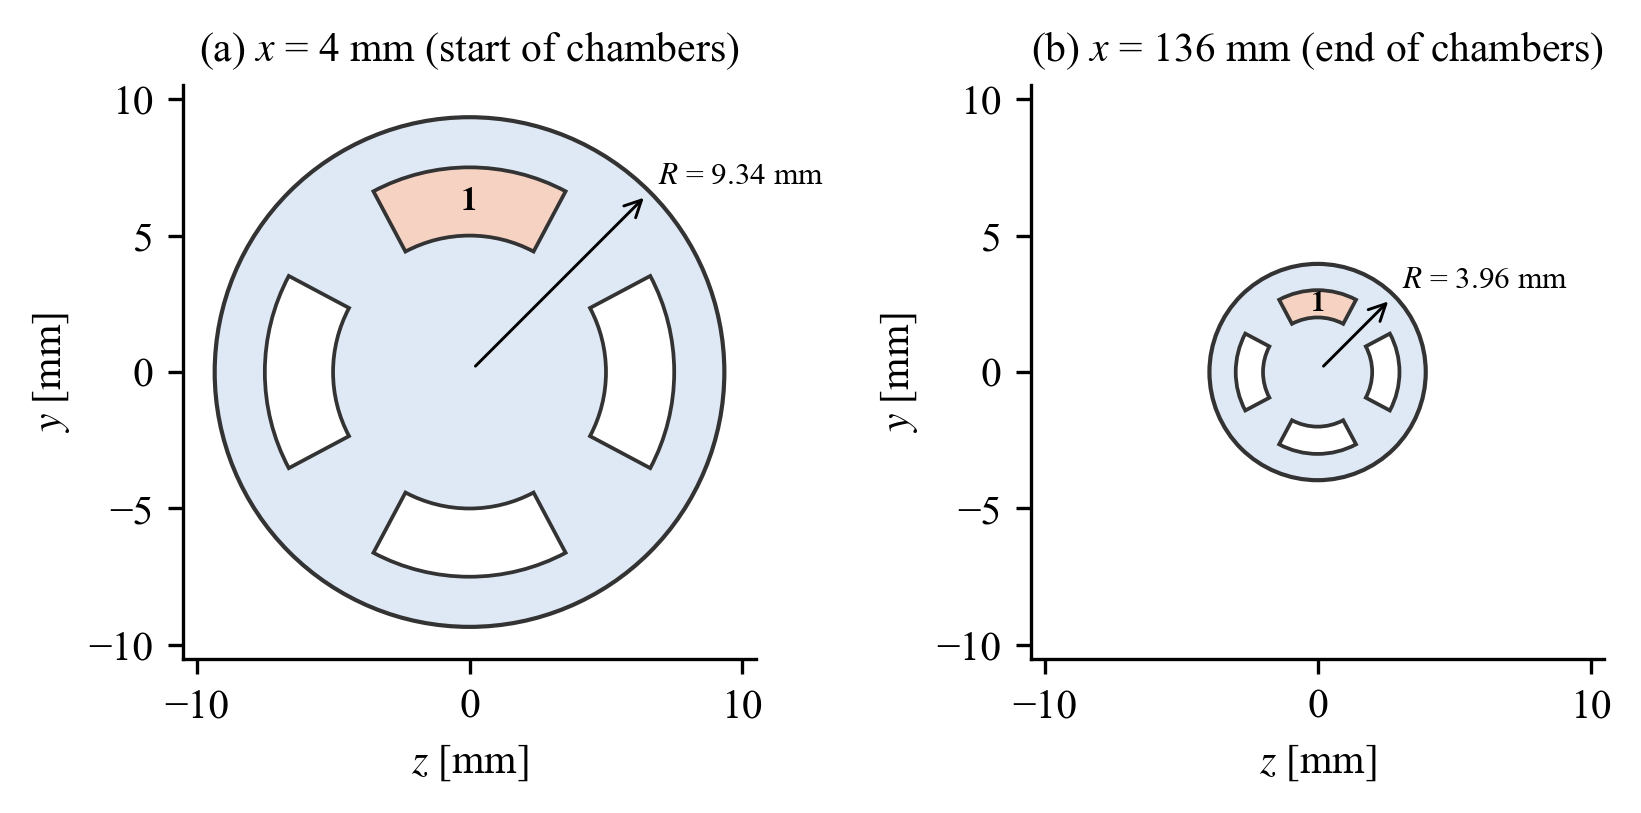
\includegraphics[width=0.78\textwidth]{fig_4ch_section.png}
\caption[Cross-section of the tapered four-chamber actuator]{Cross-section of the tapered four-chamber actuator at the two ends of the chambers (true scale).
Chamber~1 (shaded) is pressurised; the others are vented.}
\label{fig:4chsec}
\end{figure}

\begin{figure}[H]
\centering
\begin{subfigure}[b]{0.33\textwidth}\centering
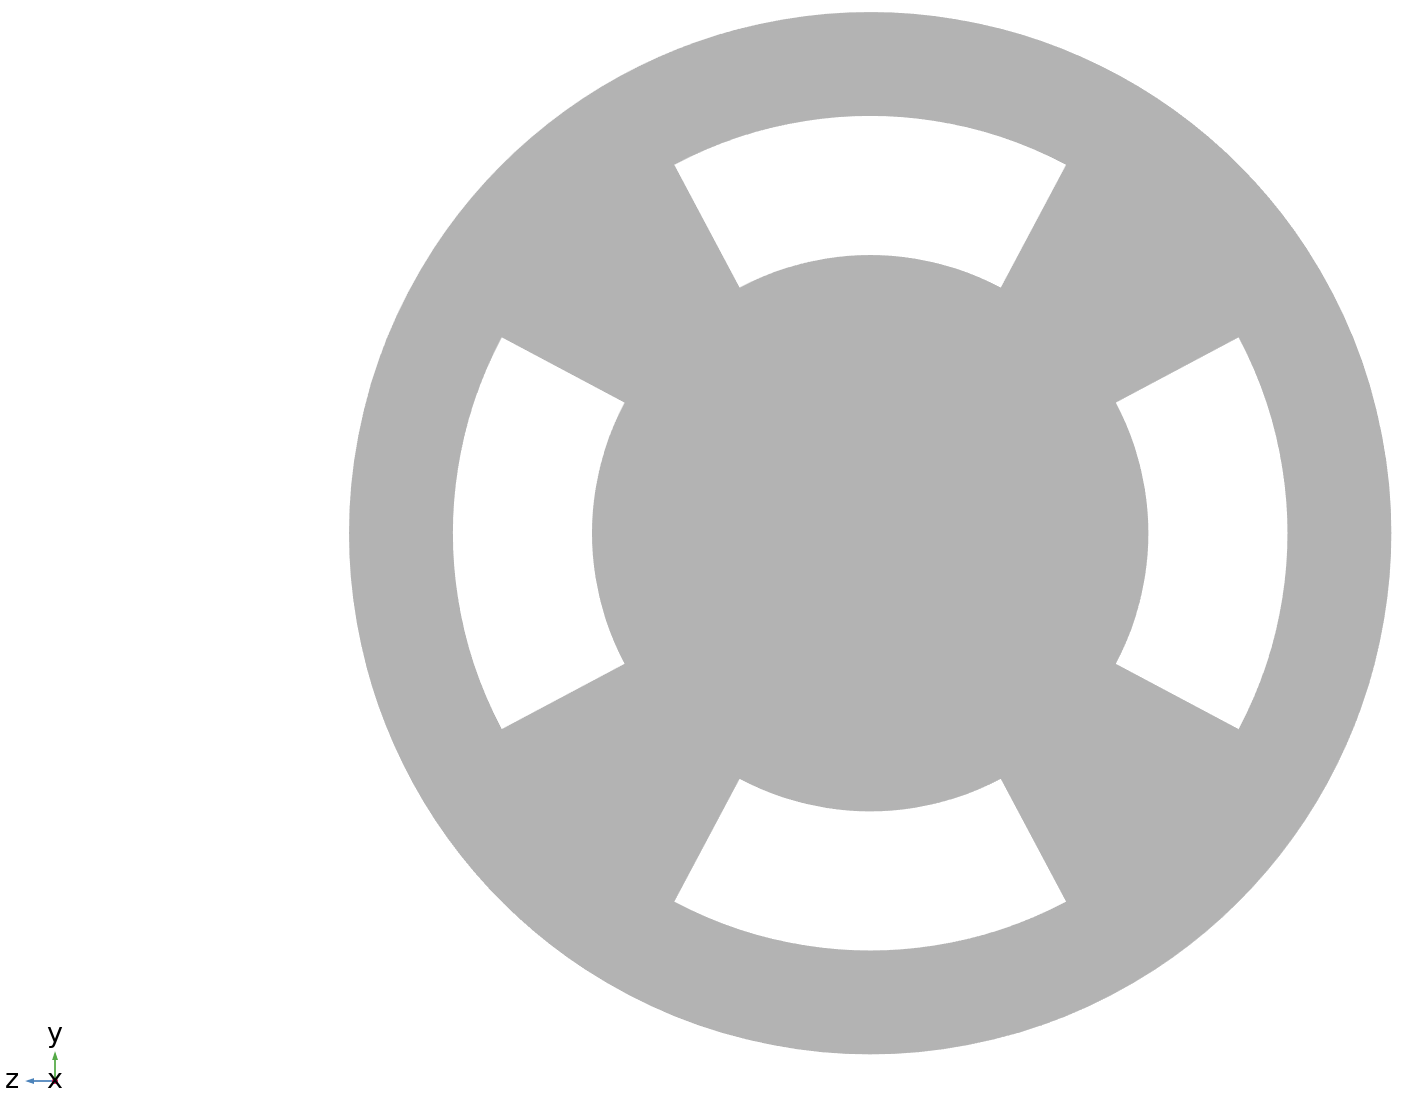
\includegraphics[width=\textwidth]{comsol_fc_sleeved_section_geom_x20.png}
\caption{$x=\SI{20}{mm}$}
\end{subfigure}\hfill
\begin{subfigure}[b]{0.283\textwidth}\centering
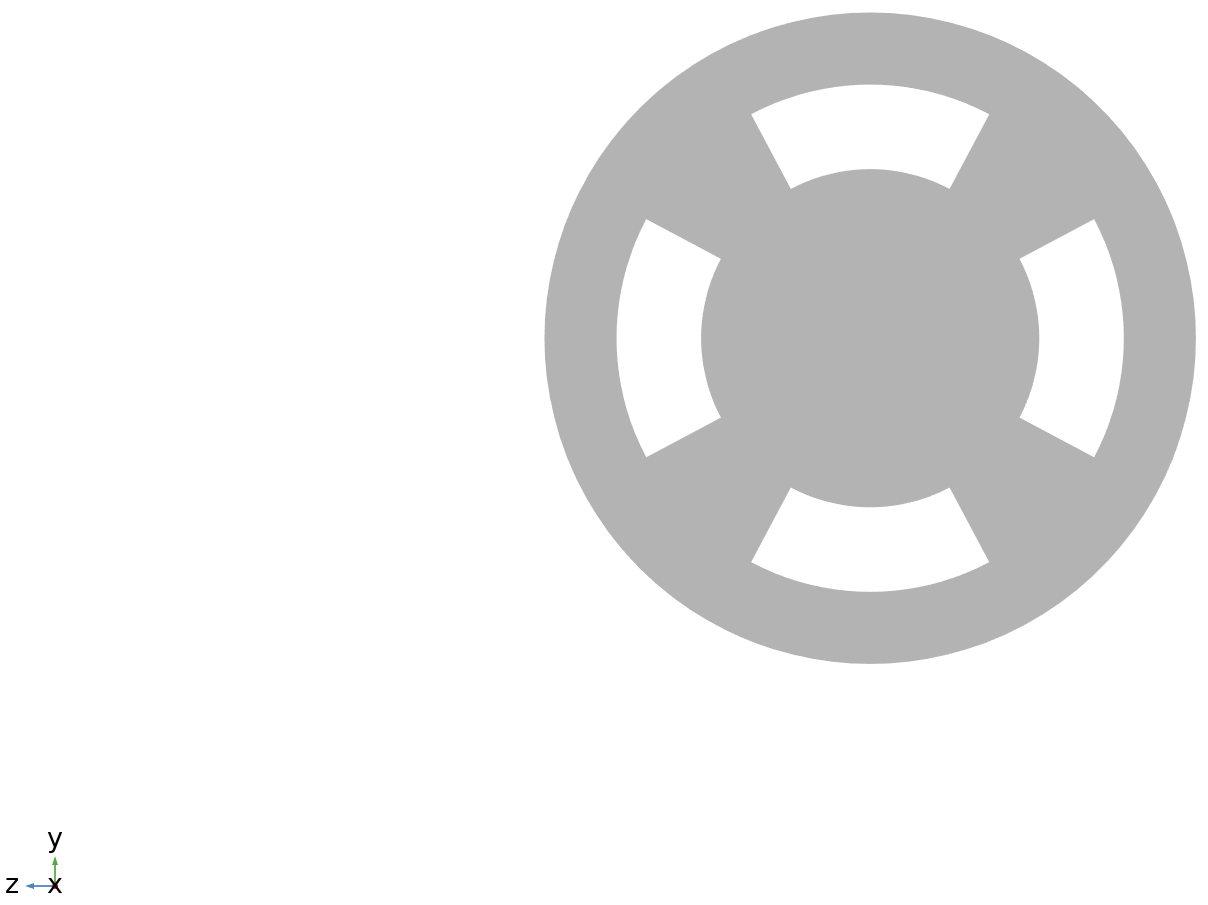
\includegraphics[width=\textwidth]{comsol_fc_sleeved_section_geom_x100.png}
\caption{$x=\SI{100}{mm}$}
\end{subfigure}\hfill
\begin{subfigure}[b]{0.33\textwidth}\centering
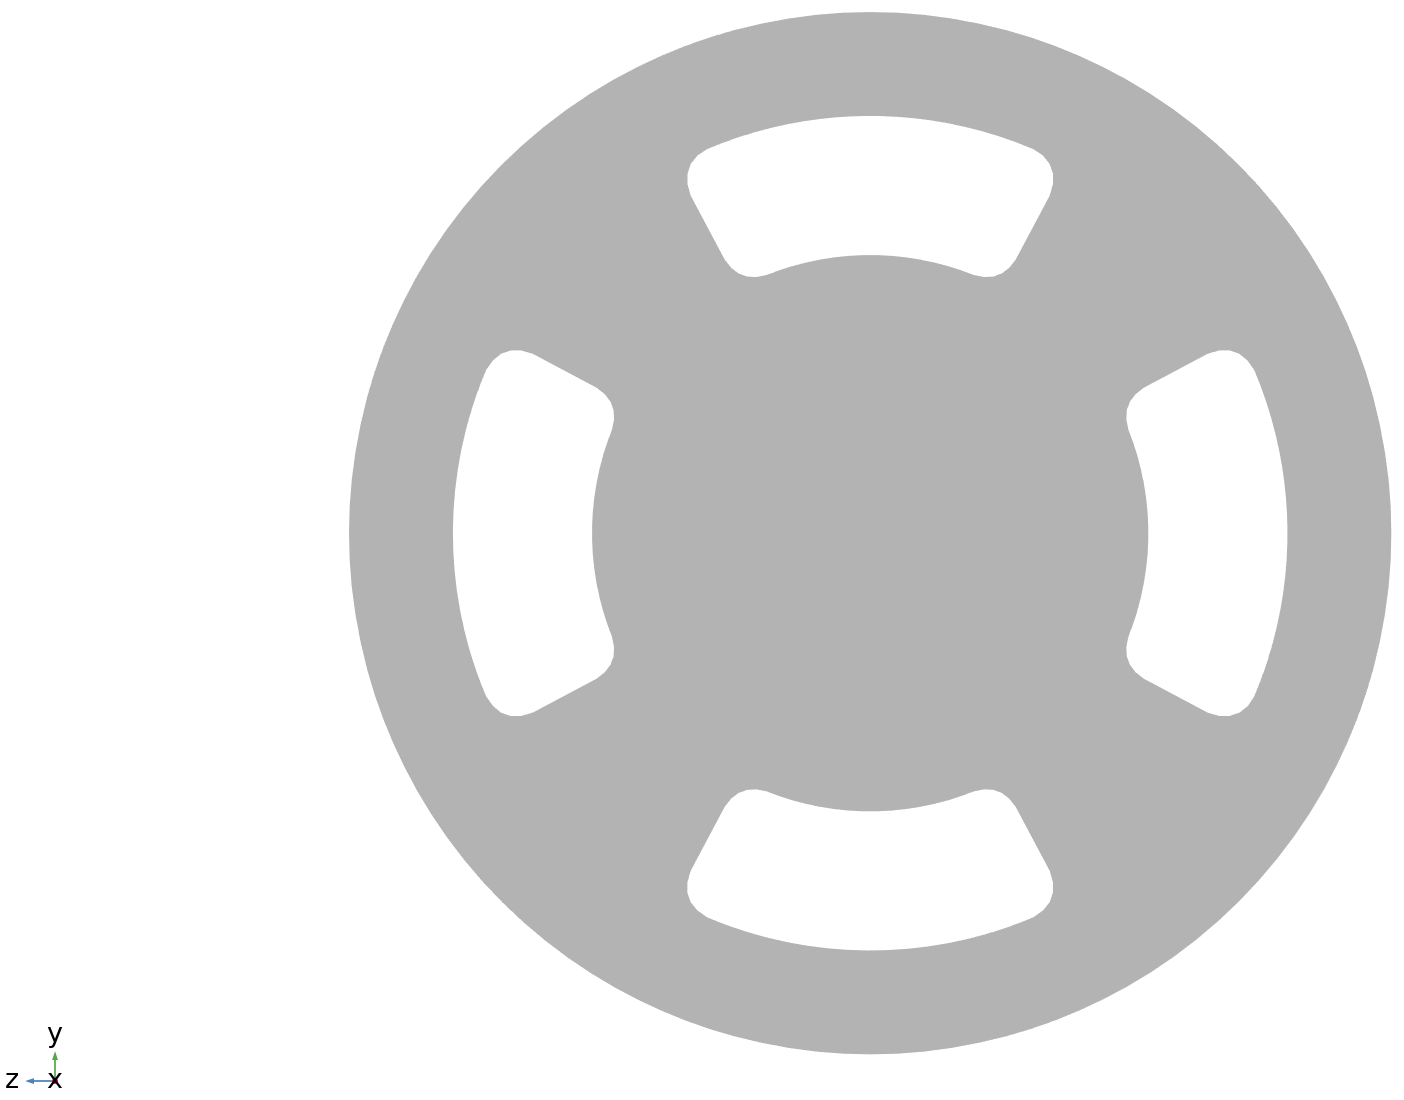
\includegraphics[width=\textwidth]{comsol_fc_fillet_section_geom_x20.png}
\caption{$x=\SI{20}{mm}$, filleted}
\end{subfigure}
\caption[COMSOL geometry of the four-chamber actuator]{Sections of the COMSOL geometry of the four-chamber actuator (undeformed), viewed along the axis
from the tip: (a), (b) original chambers at two positions, drawn at the same scale, showing the taper;
(c) the variant with \SI{0.6}{mm} fillets at the chamber corners. Chamber~1, the pressurised one, is at the top
($+y$).}
\label{fig:comsolsec}
\end{figure}

\paragraph{Selection of boundaries.} Loads and supports act on boundary faces, which must be identified
reliably. In the single-cavity model they are selected with boxes and cylinders in space (for example, all
faces lying within \SI{0.1}{mm} of the outer radius). In the four-chamber model the faces are classified
from their geometry alone: for every face the script computes its area, the mean axial position, the mean
direction from the axis and the root-mean-square distance from the outer cone. Faces at $x=0$ are the base,
faces at $x=L$ are the tip, faces within \SI{0.5}{mm} (r.m.s.) of the outer cone are the outer skin (the
r.m.s.\ distance of a true skin face is about \SI{0.06}{mm}, caused by the faceting of the curved surface,
while chamber faces are more than \SI{1.5}{mm} away), and every remaining face is assigned to the chamber in
whose direction it lies. The classification is printed and was checked for every run.

\section{Material model}
The silicone is modelled as a nearly incompressible neo-Hookean solid \cite{treloar1975,holzapfel2000}. With
the deformation gradient $\bm F$, $J=\det\bm F$ and the isochoric invariant
$\bar I_1=J^{-2/3}\,\mathrm{tr}(\bm F^{\mathsf T}\bm F)$, the strain-energy density is
\begin{equation}
W=\frac{\mu}{2}\big(\bar I_1-3\big)+\frac{\kappa_b}{2}\big(J-1\big)^2 , \label{eq:nh}
\end{equation}
which is COMSOL's neo-Hookean model with the ``nearly incompressible'' option and a quadratic volumetric
energy \cite{comsolsm}. The bulk modulus is set from Poisson's ratio,
$\kappa_b=2\mu(1+\nu)/[3(1-2\nu)]$ with $\nu=0.4995$, so that $\kappa_b\approx1000\,\mu$ and the volume of the
material hardly changes. A nearly incompressible material cannot be computed accurately with displacements
alone, because the elements become far too stiff in volume (volumetric locking). COMSOL's mixed
(``$p$-'') formulation was therefore used, in which an auxiliary pressure field is solved for together with
the displacements \cite{holzapfel2000,comsolsm}.

The moduli are placeholders. The single-cavity model uses $E=\SI{0.6}{MPa}$ ($\mu=E/3=\SI{0.2}{MPa}$), the value
used in Chapter~\ref{ch:theory}. The four-chamber model uses $E=\SI{0.07}{MPa}$ ($\mu=E/[2(1+\nu)]=\SI{23.3}{kPa}$),
an assumed value of the order of the \SI{100}{\percent} modulus of a soft platinum-cure silicone
(\SI{69}{kPa} for Ecoflex 00-30 \cite{ecoflex}); it has not been measured. For a neo-Hookean material a
change of modulus only rescales the pressure (the response depends on $P/\mu$), so these choices do not
affect the shape of the results.

\section{Supports and loads}
\begin{itemize}
\item \textbf{Base.} All displacements of the base face ($x=0$) are zero, which represents an actuator clamped
at its base.
\item \textbf{Symmetry} (single-cavity model only). The displacement normal to the plane $z=0$ is zero.
\item \textbf{Cavity pressure.} A gauge pressure $P$ acts on every face of the pressurised cavity: the
cavity wall and the inner face of the tip cap, and, for the four-chamber model, every face of chamber~1. It
is applied as a \emph{follower} pressure, which acts normal to the deformed surface and on its deformed
area \cite{comsolsm}, as the pressure of a gas or liquid does. The other three chambers of the four-chamber
actuator are vented (no load). Gravity is neglected.
\end{itemize}

\paragraph{Hoop sleeve.} A sleeve of circumferential fibres around the outer surface is modelled as a
surface energy on the outer skin, added through COMSOL's \emph{weak contribution} feature, which adds a
user-written term to the weak (virtual-work) form of the equations \cite{comsol}. In reference
coordinates $(X,Y,Z)$ the hoop direction is the unit vector $\bm t=(0,-Z,Y)/\sqrt{Y^2+Z^2}$, and the Green
strain of the surface along $\bm t$ is \cite{holzapfel2000}
\begin{equation}
e_h=\tfrac12\big(\lambda_h^2-1\big)=\bm t\cdot\big(\nabla\bm u\big)\bm t+\tfrac12\big|\big(\nabla\bm u\big)\bm t\big|^2 ,
\qquad \lambda_h=|\bm F\bm t| ,
\end{equation}
where $\bm u$ is the displacement. Only derivatives tangential to the surface are needed, because $\bm t$ lies
in the surface. The sleeve stores the energy $\tfrac12 k_s e_h^2$ per unit reference area, i.e.\ the weak
contribution $-k_s\,e_h\,\delta e_h$ integrated over the outer skin. The sleeve therefore resists hoop
stretching only; it has no axial and no bending stiffness and is perfectly bonded to the silicone. The stiffness
$k_s=100\,ER$ ($R$ at the base for the tapered actuator) is a penalty value, chosen to be much larger than
the hoop membrane stiffness of the silicone wall (of order $Et$ with wall thickness $t<R$), so that the
sleeve is nearly inextensible. Because $\bm t$ is tangent to a cone as well as to a cylinder, the same
formulation applies to the tapered actuator.

\section{Mesh}
Both models use a free tetrahedral mesh generated automatically with COMSOL's ``Fine'' size preset, with
quadratic displacement shape functions. The four-chamber mesh has 18\,044 elements (20\,946 for the deeper
chambers and 36\,362 with fillets, which need small elements to resolve the rounded corners).
Figure~\ref{fig:mesh} shows the surface of the two meshes near the base.

\begin{figure}[H]
\centering
\begin{subfigure}[b]{0.49\textwidth}\centering
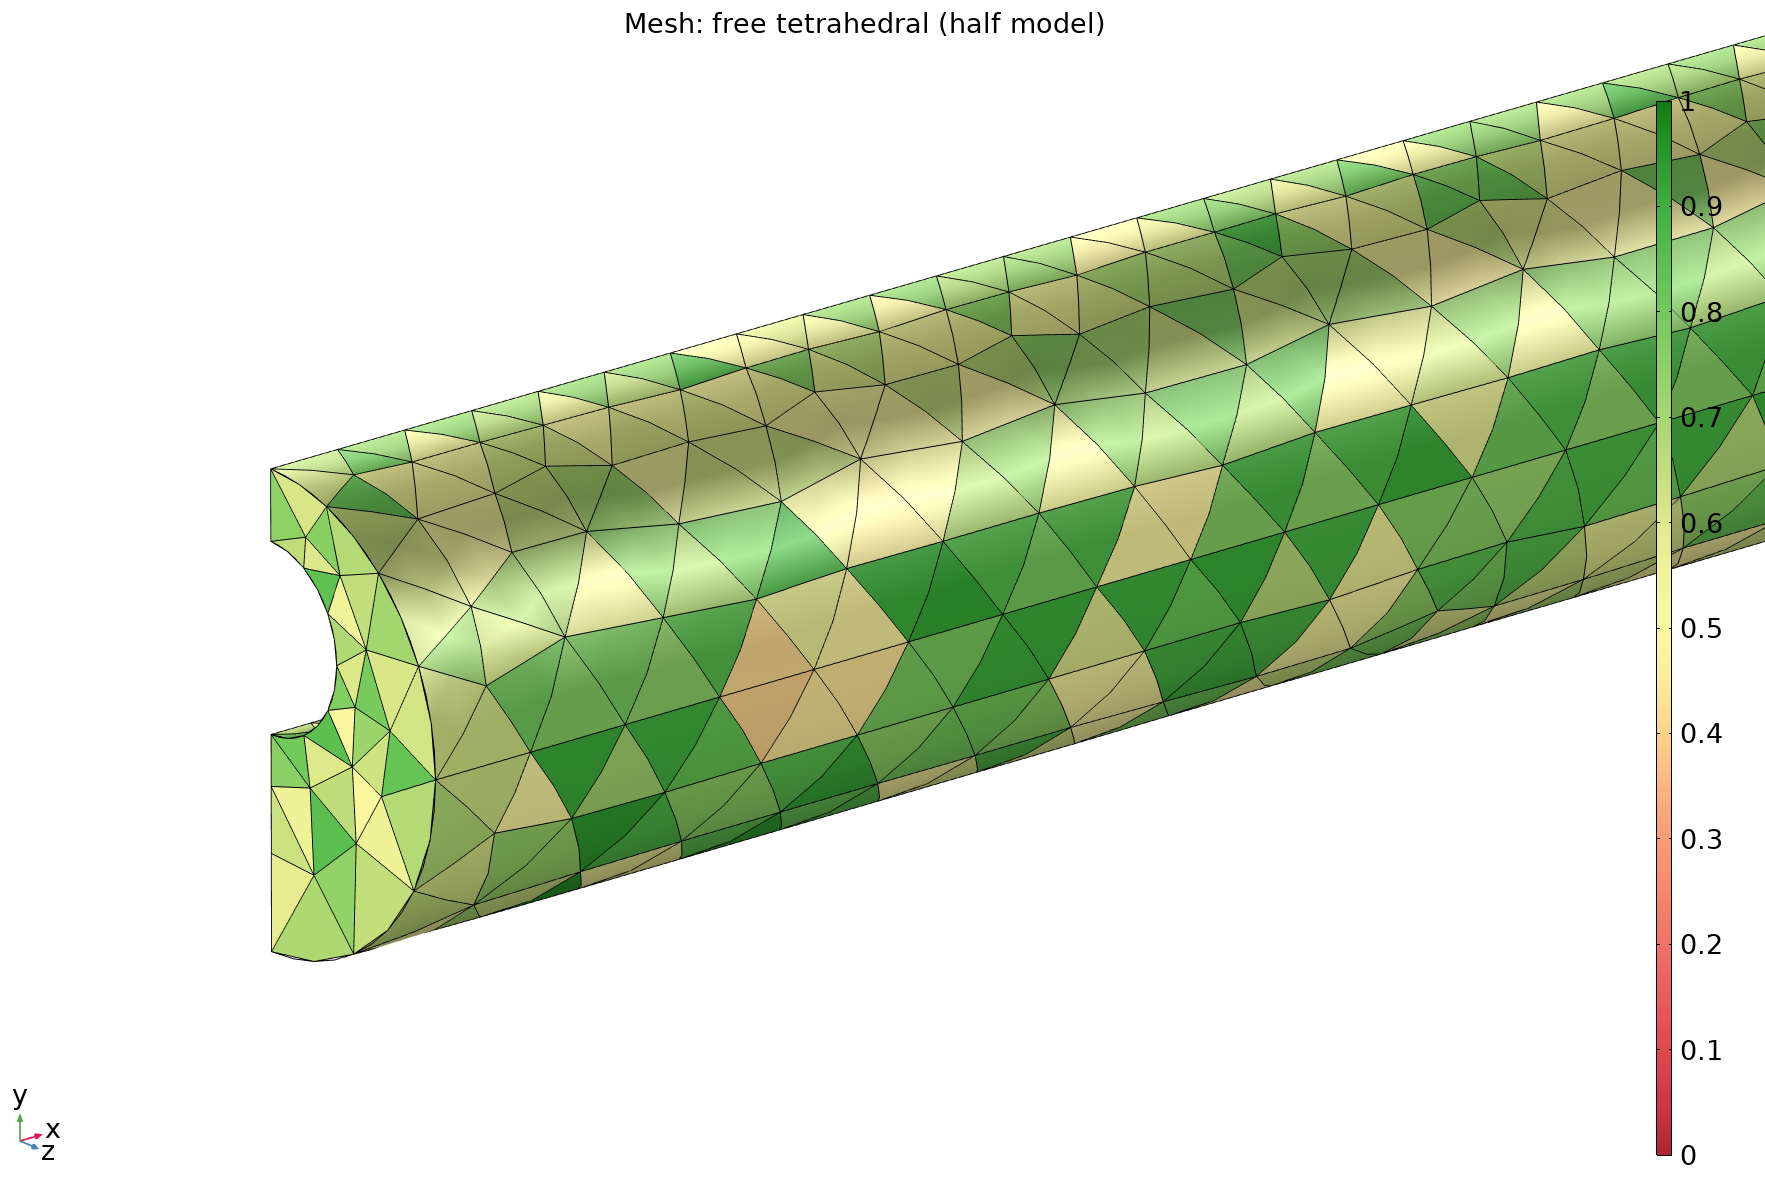
\includegraphics[width=\textwidth]{comsol_sc_sleeved_mesh.png}
\caption{single-cavity actuator (half model)}
\end{subfigure}\hfill
\begin{subfigure}[b]{0.49\textwidth}\centering
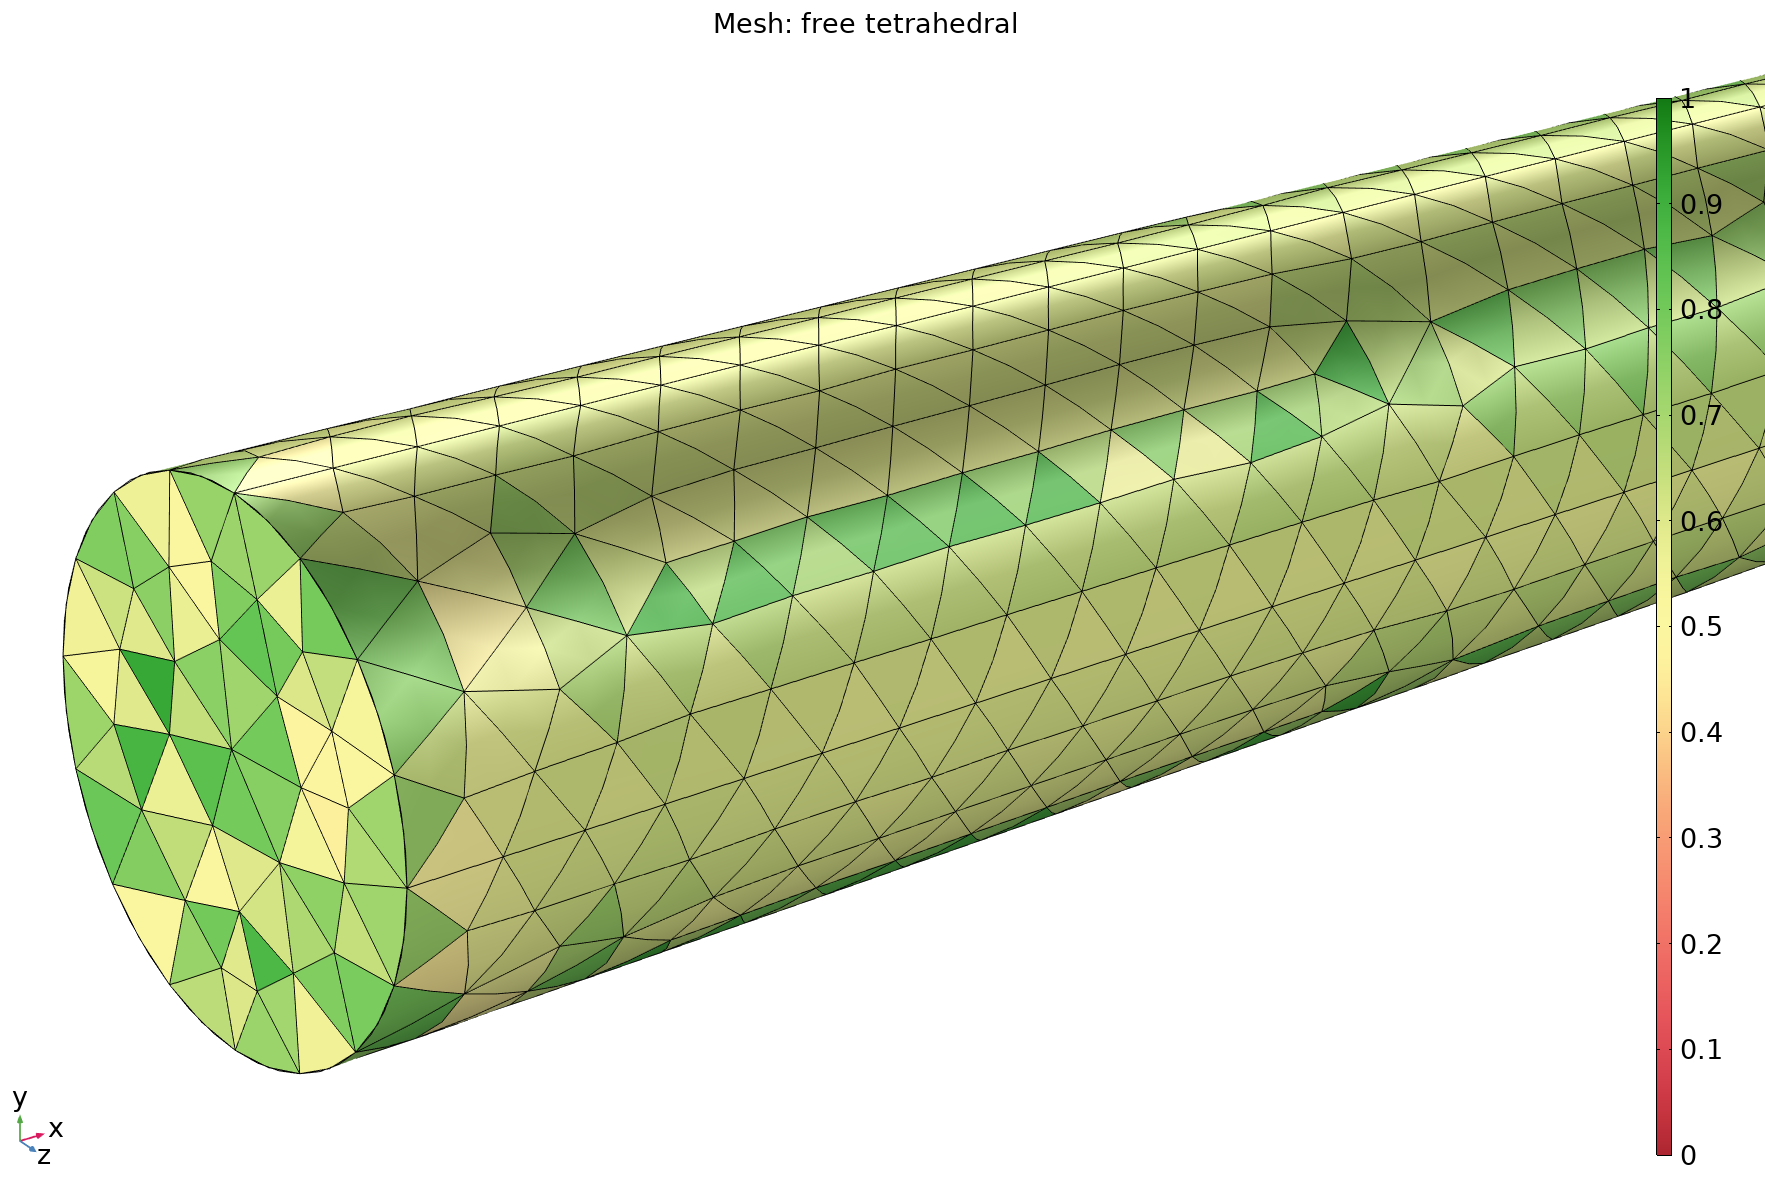
\includegraphics[width=\textwidth]{comsol_fc_sleeved_mesh.png}
\caption{four-chamber actuator}
\end{subfigure}
\caption[COMSOL meshes]{COMSOL meshes near the base ($x=0$ at the left end). (a) is the half model, cut at the symmetry
plane $z=0$; the notch at the left end is the cavity opening at the base. The elements are coloured by COMSOL's element-quality
measure, from 0 (degenerate) to 1 (ideal).}
\label{fig:mesh}
\end{figure}

\section{Solution procedure}
A stationary study with geometric nonlinearity (large deformation) was used. The pressure is increased in a
parametric sweep, each step starting from the converged solution of the previous one: \SIrange{0}{110}{kPa}
in steps of \SI{10}{kPa} for the sleeved single-cavity actuator, \SIrange{0}{90}{kPa} for the bare one, and
\SIrange{0}{100}{kPa} for the four-chamber actuator with steps of \SIrange{2}{2.5}{kPa} below \SI{30}{kPa}.
Each step is solved with COMSOL's Newton-type nonlinear solver; when a step does not converge, the solver
tries smaller intermediate pressure increments. When even these fail, the run stops and all steps converged
so far are kept; the last of them is reported as the ``last converged step''. On the project computer one
four-chamber run took between \SI{3}{min} (bare) and \SI{57}{min} (with fillets).

\section{Quantities extracted}
\paragraph{Single-cavity actuator.} The tip angle is the rotation of the line joining the two outer-surface
points at the end of the cavity, $(x,y,z)=(100,\pm10,0)$\,mm: $\theta=\arctan(\Delta x/\Delta y)$ from their
deformed positions. The tip deflection $\delta$ is minus the mean $y$-displacement of the two points.

\paragraph{Four-chamber actuator.} Tip rotation: angle of the deformed material line joining the points
$y=\pm\SI{1.5}{mm}$ at $x=\SI{139.8}{mm}$, followed continuously from step to step so that rotations beyond
\ang{90} are counted correctly. Deformed centreline: 29 points on the axis, which lies in the solid core.
Section change: deformed distance between the two outer-skin points on the $y$ axis at $x=\SI{70}{mm}$,
divided by the original diameter. The peak von Mises stress and the smallest local volume ratio $J$ over
the whole body are recorded at every step as indicators of local distortion.

\section{Mesh check}
With the ``Fine'' mesh preset replaced by ``Finer'', the tip rotation of the sleeved
four-chamber actuator at \SI{10}{kPa} changes by 1.2\,\% (\ang{47.1} to \ang{47.7}) and the tip deflection by
0.9\,\%. The check was not repeated at higher pressure, and no mesh check was made for the single-cavity
model.

\section{Beam estimate for the tapered actuator}
For comparison, eq.~(\ref{eq:kappa}) was integrated over the tapered section. A chamber is an annular sector
of half-angle $\alpha$ between radii $a(x)$ and $b(x)$, with area $A_c=\alpha(b^2-a^2)$ and centroid at
$e=\frac{2\sin\alpha}{3\alpha}\frac{b^3-a^3}{b^2-a^2}$ from the axis.\footnote{By integration in polar
coordinates: $A_c=\int_{-\alpha}^{\alpha}\!\int_a^b\rho\,d\rho\,d\varphi$ and
$A_c e=\int_{-\alpha}^{\alpha}\!\int_a^b\rho\cos\varphi\,\rho\,d\rho\,d\varphi=\tfrac23\sin\alpha\,(b^3-a^3)$; see the
tables of centroids in \cite{gere2013}.} The free-body argument of Section~\ref{sec:load} gives
$M(x)=PA_c(x)e(x)$ at each section, and the section with four equal voids has its centroid on the axis and
$I=\pi R^4/4-\alpha(b^4-a^4)$ about it,\footnote{A sector contributes
$\int\!\!\int\rho^2\sin^2\varphi\,\rho\,d\rho\,d\varphi$; for four sectors \ang{90} apart the angular integrals
add up to $4\alpha$, so the four voids remove $\tfrac14(b^4-a^4)\cdot4\alpha$ from the solid disc.} so
\begin{equation}
\theta_{\text{beam}} = \frac{P}{E}\int_{x_s}^{x_e}\frac{A_c(x)\,e(x)}{I(x)}\,dx . \label{eq:taper}
\end{equation}
Like eq.~(\ref{eq:theta}), this applies to a hoop-reinforced actuator at small $P/E$; the solid plug and
cap are treated as rigid.

% =====================================================================
\chapter{Results}\label{ch:results}
% =====================================================================

\section{Single-cavity actuator}\label{sec:res1}
Table~\ref{tab:fe} and Figure~\ref{fig:response} compare the COMSOL results with the beam model,
eqs.~(\ref{eq:theta}) and (\ref{eq:delta}), for the placeholder design ($E=\SI{0.6}{MPa}$, $\mu=\SI{0.2}{MPa}$).

\begin{table}[H]
\centering\small
\caption[Single-cavity actuator: COMSOL and beam model]{Single-cavity actuator, $E=\SI{0.6}{MPa}$: tip angle $\theta$ and tip deflection $\delta$ from COMSOL,
and the ratio of the COMSOL tip angle to the beam model. The bare run ends at \SI{90}{kPa}, the last pressure
requested. For another neo-Hookean silicone the pressure scales with $\mu$.}
\label{tab:fe}
\begin{tabular}{@{}rccccccc@{}}
\toprule
& & \multicolumn{3}{c}{Bare} & \multicolumn{3}{c}{Hoop-reinforced (sleeved)}\\
\cmidrule(lr){3-5}\cmidrule(lr){6-8}
$P$ [kPa] & $\theta_{\text{beam}}$ [\si{\degree}] & $\theta$ [\si{\degree}] & FE/beam & $\delta$ [mm] & $\theta$ [\si{\degree}] & FE/beam & $\delta$ [mm]\\
\midrule
10 & 2.41 & 0.263 & 0.11 & 0.22 & 2.43 & 1.01 & 2.12\\
20 & 4.82 & 0.761 & 0.16 & 0.64 & 5.06 & 1.05 & 4.44\\
40 & 9.64 & 2.78 & 0.29 & 2.37 & 11.0 & 1.15 & 9.83\\
60 & 14.5 & 7.12 & 0.49 & 6.12 & 18.2 & 1.26 & 16.4\\
80 & 19.3 & 16.6 & 0.86 & 14.4 & 26.7 & 1.39 & 24.3\\
90 & 21.7 & 26.0 & 1.20 & 22.6 & 31.6 & 1.46 & 28.9\\
100 & 24.1 & -- & -- & -- & 37.0 & 1.54 & 34.0\\
110 & 26.5 & -- & -- & -- & 43.0 & 1.62 & 39.5\\
\bottomrule
\end{tabular}
\end{table}

\begin{figure}[H]
\centering
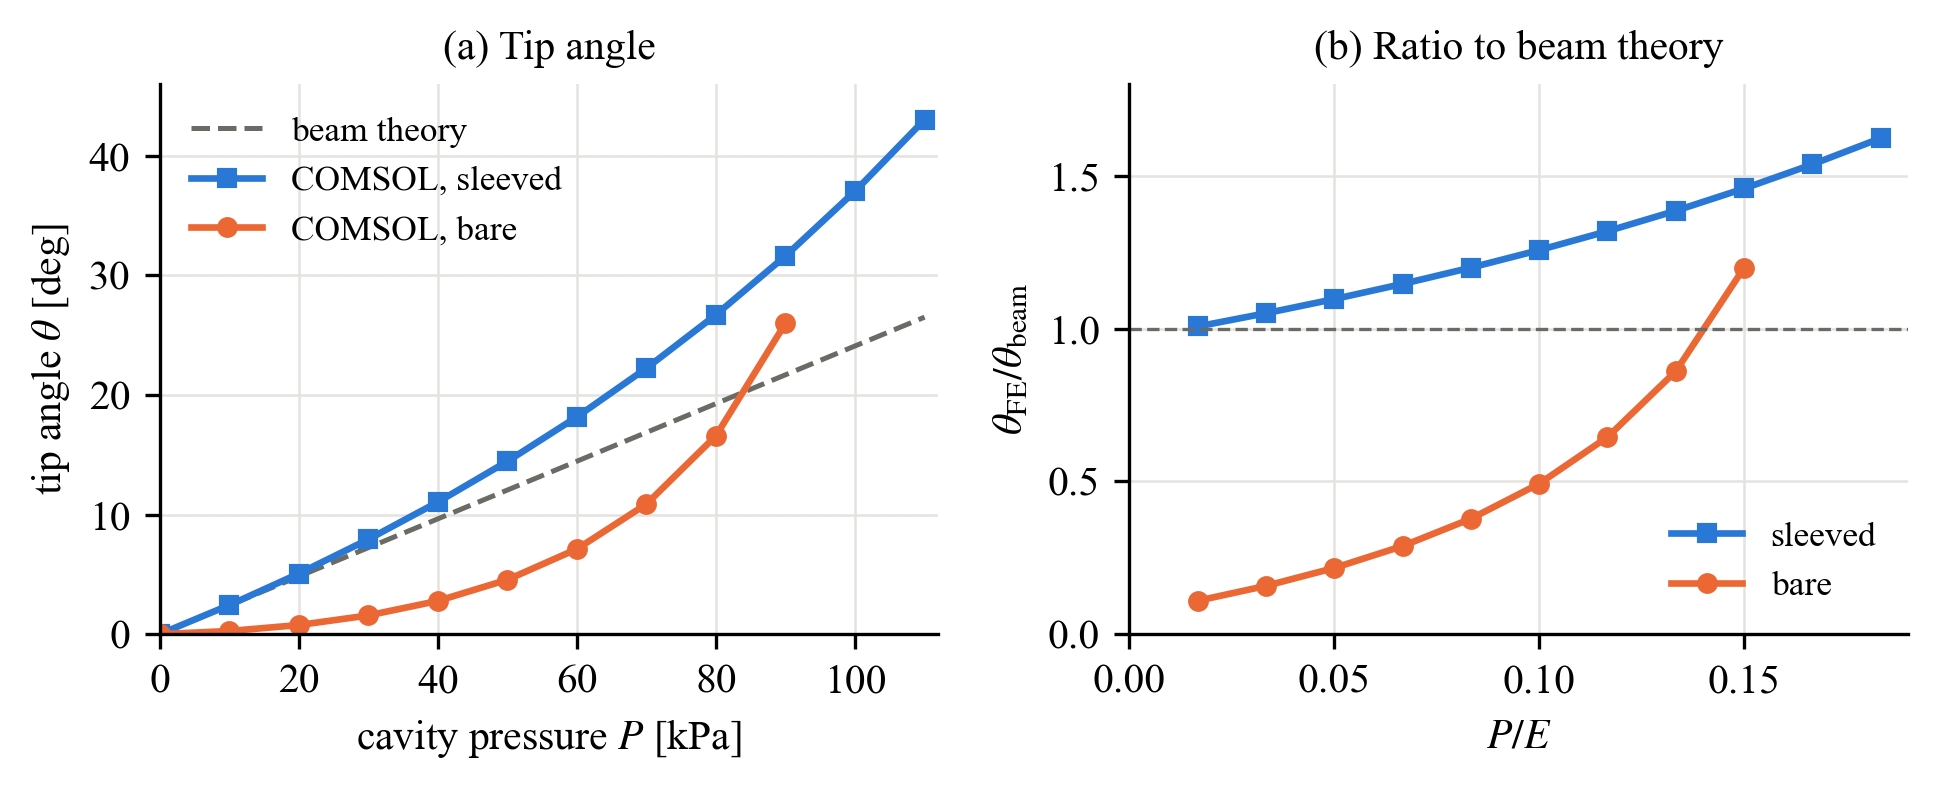
\includegraphics[width=\textwidth]{fig_single_cavity.png}
\caption[Single-cavity actuator: COMSOL and beam model]{Single-cavity actuator: (a) tip angle against pressure from the beam model, eq.~(\ref{eq:theta}),
and from COMSOL, bare and sleeved; (b) ratio of the COMSOL tip angle to the beam model against $P/E$.}
\label{fig:response}
\end{figure}

\paragraph{Hoop-reinforced actuator.} The response is smooth up to \SI{110}{kPa}, the last pressure
requested, and every requested step converged. At small pressure it agrees with the beam model: the
ratio of the tip angles is 1.01 at $P/E=0.017$ (\SI{10}{kPa}) and 1.05 at $P/E=0.033$ (\SI{20}{kPa}). Since
eq.~(\ref{eq:theta}) and the FE model share only the geometry, the modulus and the pressure, this agreement is
also an independent check of the FE model set-up (geometry, material, follower load and the way the tip
angle is measured). At higher pressure the FE model bends more than the beam model, by 26\,\% at $P/E=0.1$
and 62\,\% at \SI{110}{kPa}. The beam model uses the undeformed section and a linear material, whereas the FE
model follows the change of geometry with pressure; the separate contributions of these effects were not
determined.

\paragraph{Bare actuator.} The bare actuator bends far less than the beam model at small pressure: 11\,\% of
it at \SI{10}{kPa} and 16\,\% at \SI{20}{kPa}. This is the reduction predicted by eq.~(\ref{eq:poisson}). The
remaining bending is not zero; these runs do not separate the second-order mechanism of
eq.~(\ref{eq:twothirds}) from the effect of the two ends, where the clamp and the cap restrain the wall and
the in-plane stress state of Section~\ref{sec:poisson} does not hold. The tip angle grows faster than
linearly with pressure (by a factor of 2.9 from 10 to \SI{20}{kPa} and 3.7 from 20 to \SI{40}{kPa}), as expected
of a mechanism that is quadratic in the hoop strain. The FE and beam curves cross between 80 and
\SI{90}{kPa}; this is a coincidence of two different mechanisms, not an agreement. Between 80 and
\SI{90}{kPa} the deflection increases by \SI{8.2}{mm}, against \SI{5.0}{mm} between 70 and \SI{80}{kPa}, so
the response is steepening, as expected on the approach to ballooning (Section~\ref{sec:wall}). The run ends
at \SI{90}{kPa}, so the limit pressure itself was not reached.

\paragraph{Deformed shapes.} Figure~\ref{fig:scside} shows the two actuators at \SI{40}{kPa} and
\SI{90}{kPa} with the same colour scale, and Figure~\ref{fig:scsection} the section at mid-length at
\SI{90}{kPa}. At \SI{40}{kPa} the bare actuator is still almost straight (\ang{2.8}), while the sleeved one has
bent by \ang{11}. At \SI{90}{kPa} the cavity of the bare actuator has grown far more than that of the sleeved
one, and the von Mises stress is highest in the material around the cavity; in the sleeved actuator the
outer boundary of the section stays circular, because the sleeve prevents it from stretching in the hoop
direction.

\begin{figure}[htbp]
\centering
\begin{subfigure}[b]{0.49\textwidth}\centering
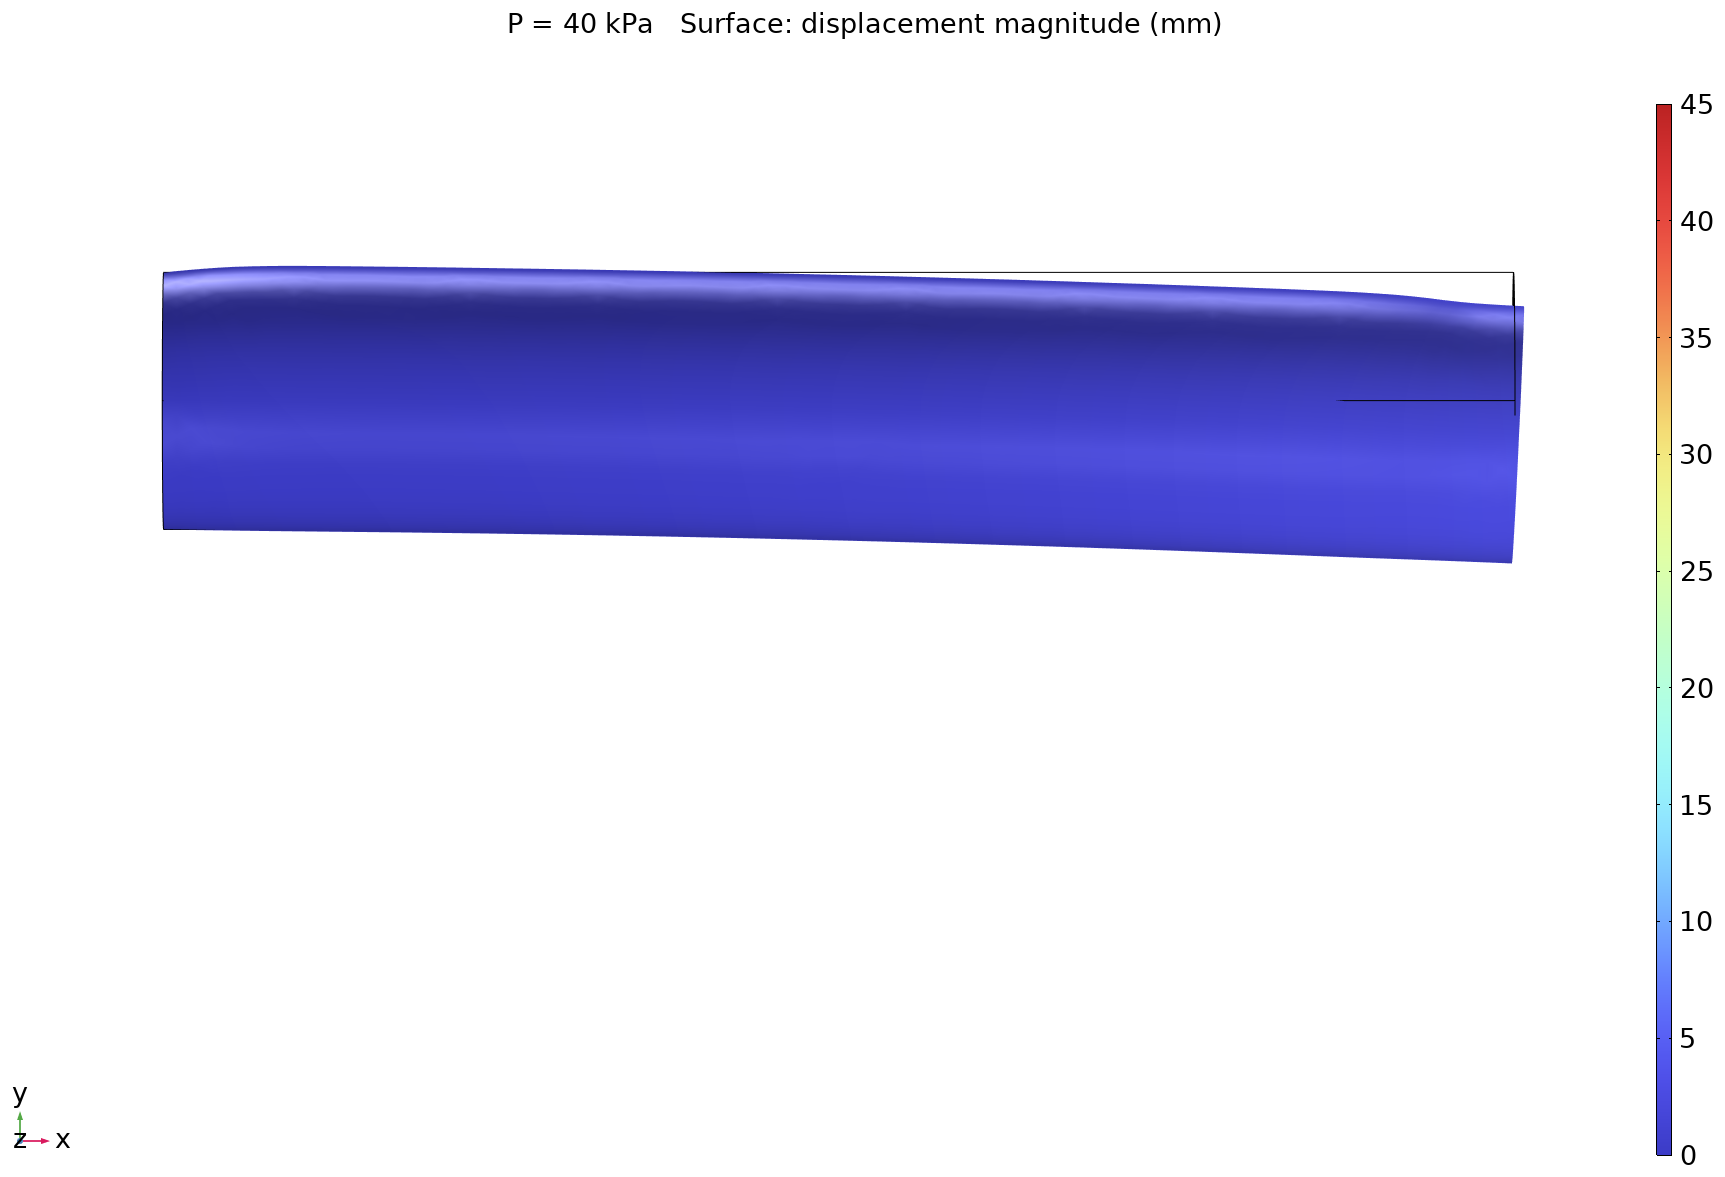
\includegraphics[width=\textwidth]{comsol_sc_bare_side_P40.png}
\caption{bare, \SI{40}{kPa}}
\end{subfigure}\hfill
\begin{subfigure}[b]{0.49\textwidth}\centering
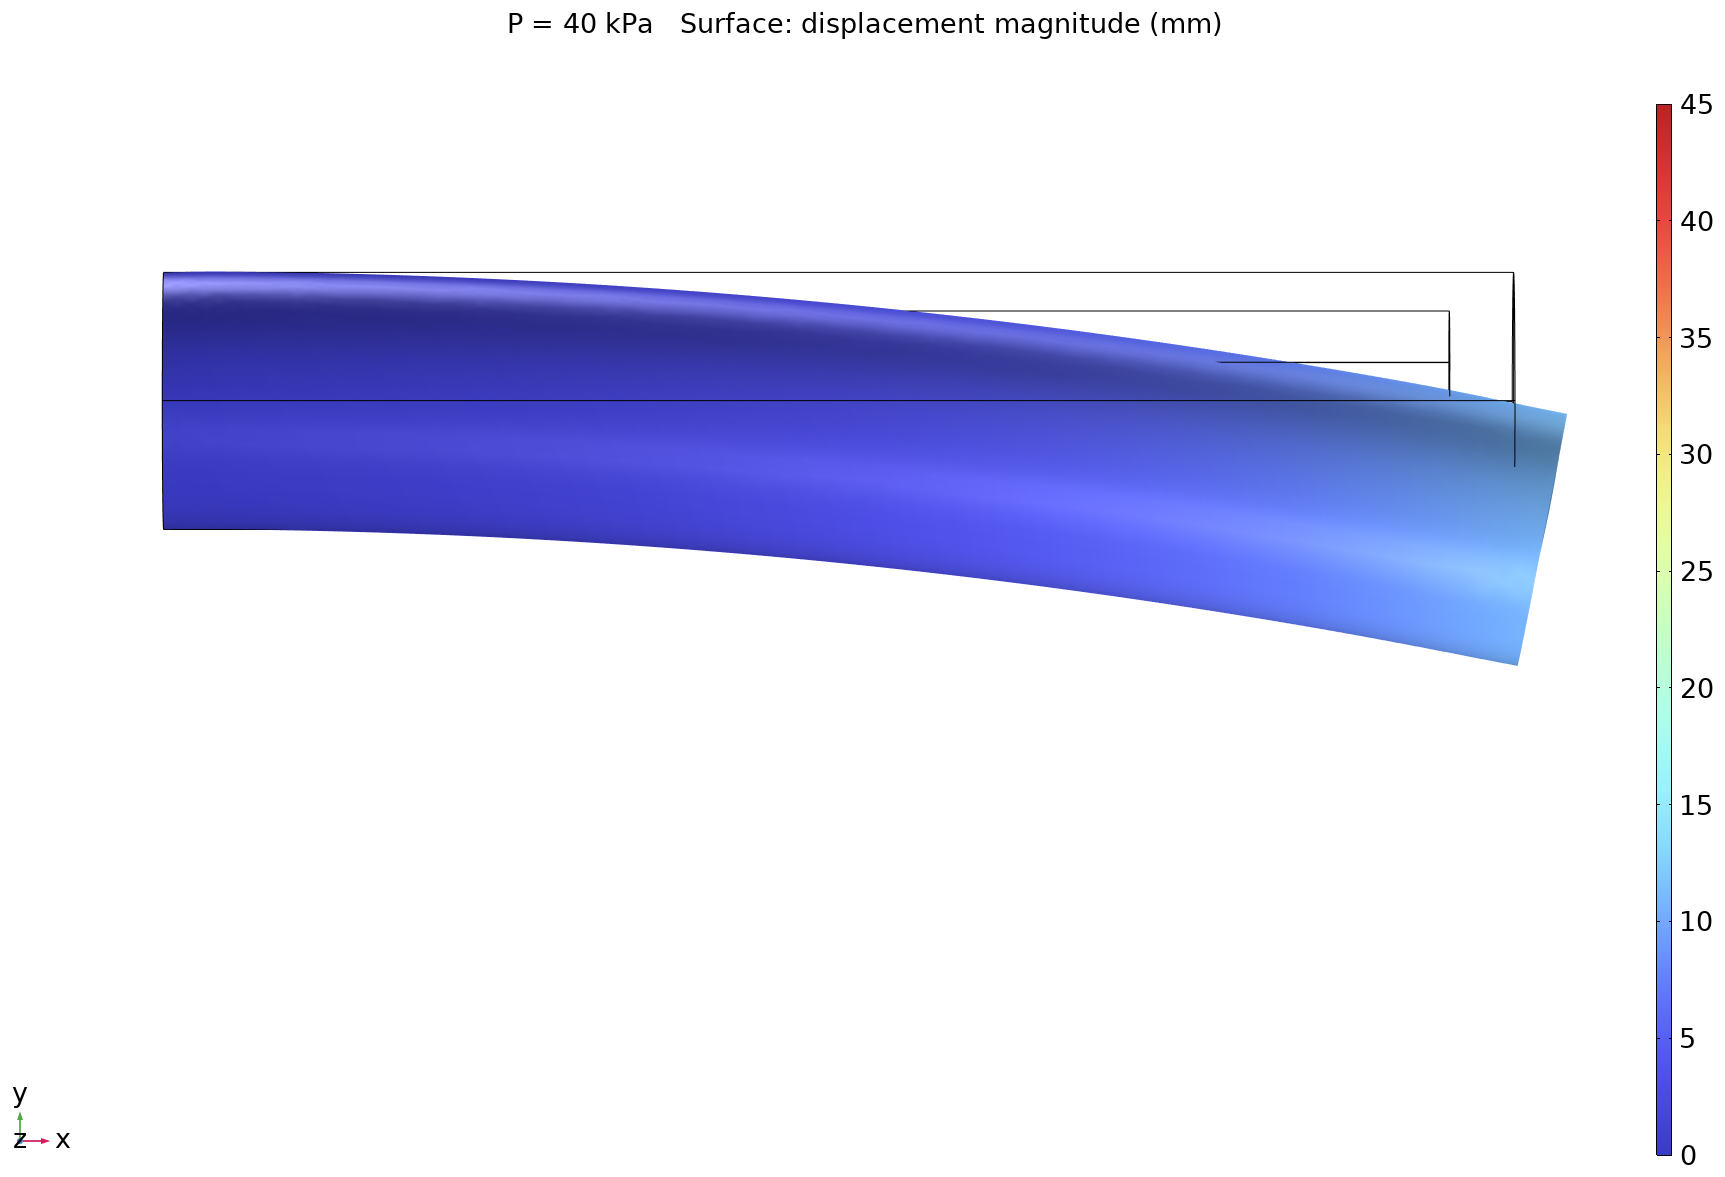
\includegraphics[width=\textwidth]{comsol_sc_sleeved_side_P40.png}
\caption{sleeved, \SI{40}{kPa}}
\end{subfigure}

\vspace{4pt}
\begin{subfigure}[b]{0.49\textwidth}\centering
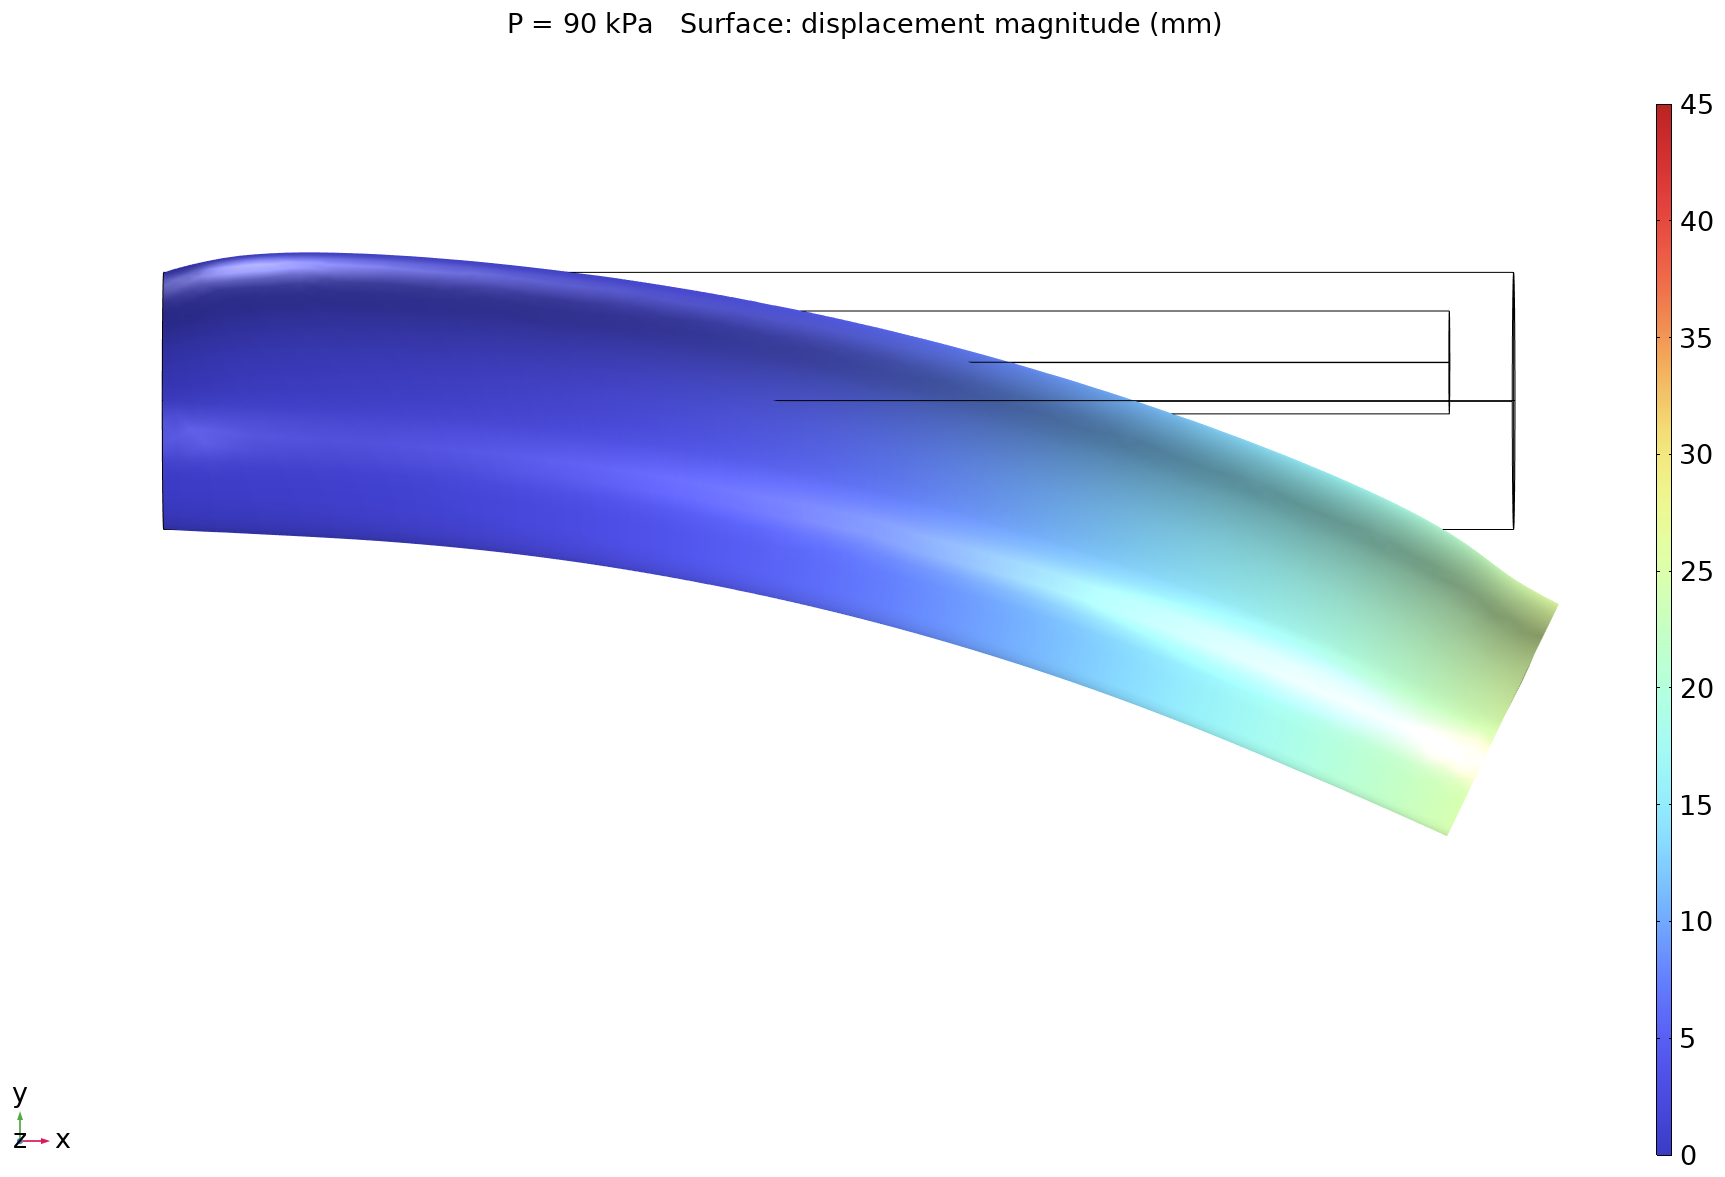
\includegraphics[width=\textwidth]{comsol_sc_bare_side_P90.png}
\caption{bare, \SI{90}{kPa}}
\end{subfigure}\hfill
\begin{subfigure}[b]{0.49\textwidth}\centering
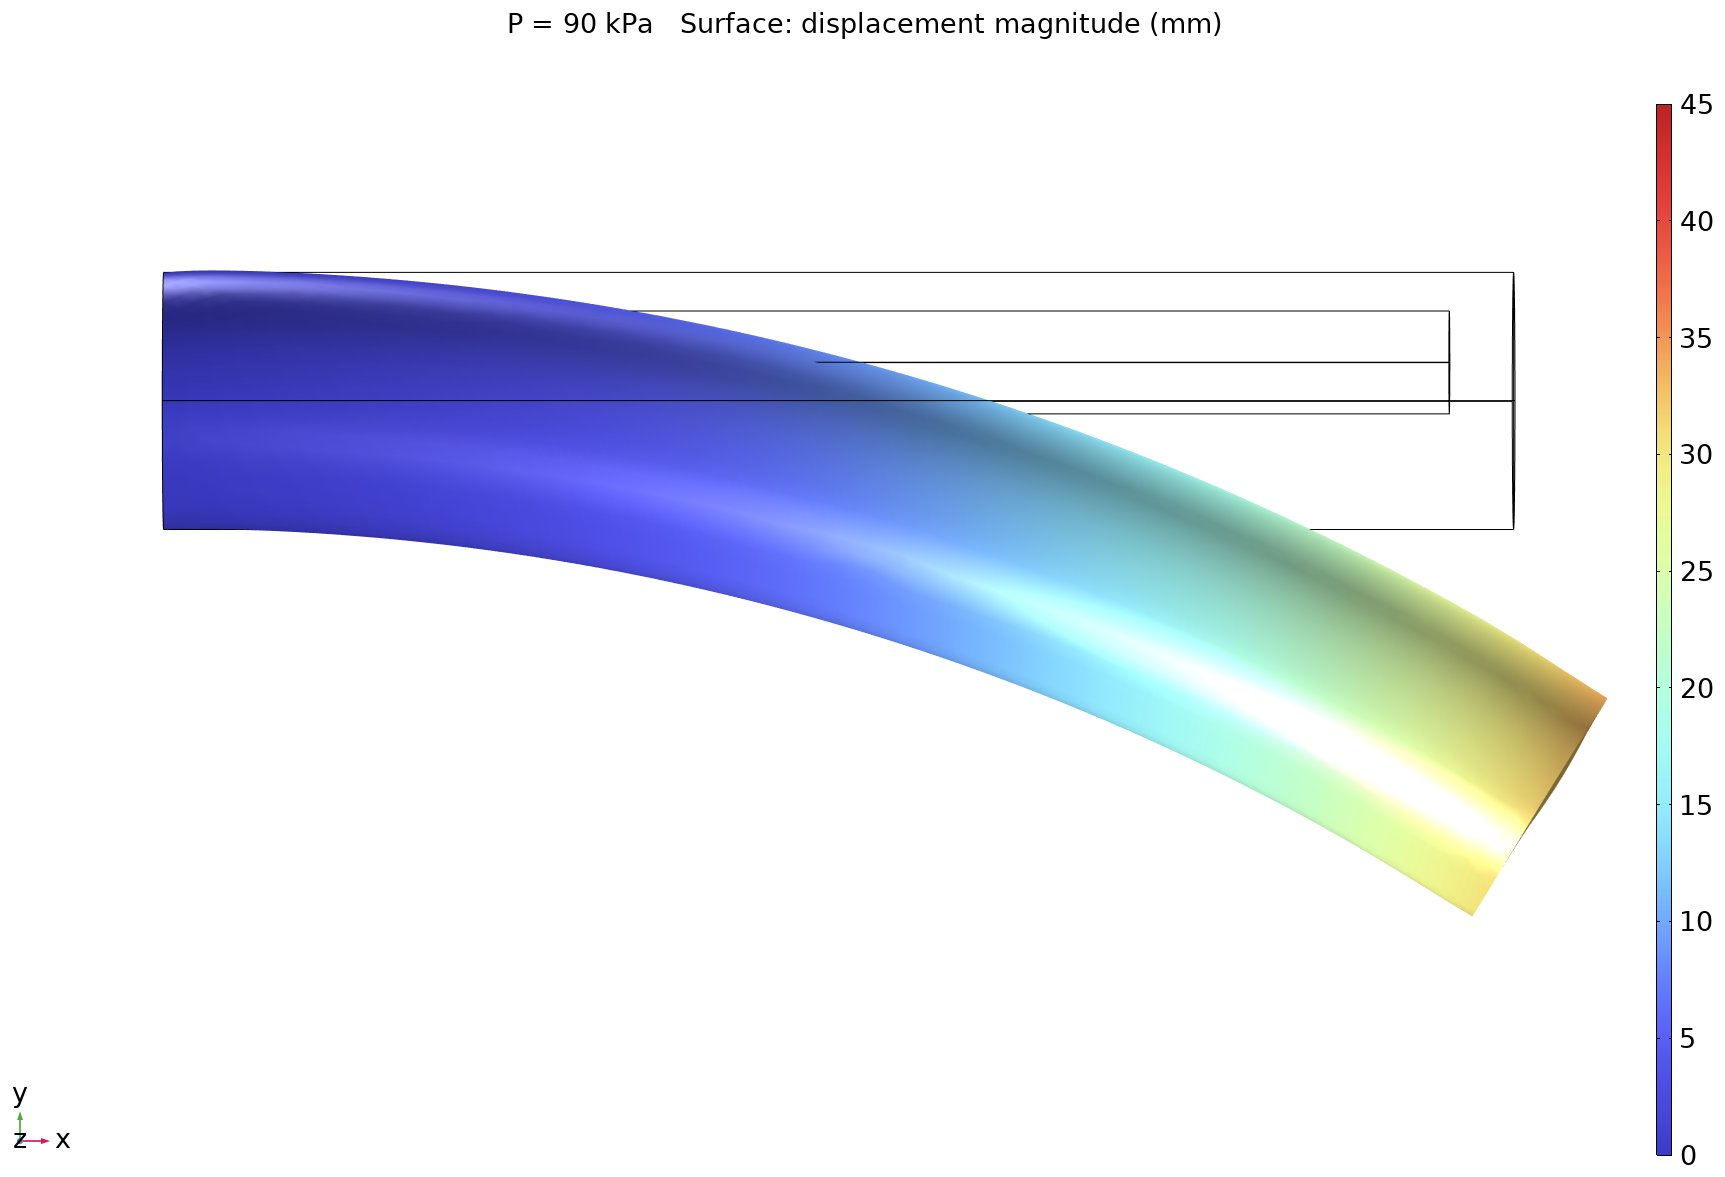
\includegraphics[width=\textwidth]{comsol_sc_sleeved_side_P90.png}
\caption{sleeved, \SI{90}{kPa}}
\end{subfigure}
\caption[Single-cavity actuator: deformed shapes (COMSOL)]{Single-cavity actuator, $E=\SI{0.6}{MPa}$: deformed shape viewed normal to the bending plane
(COMSOL, true scale; the half model is mirrored about $z=0$ for display). Colour: displacement magnitude
[mm], same scale (0--45~mm) in all four panels. The thin lines show the undeformed body; the base is clamped
at the left.}
\label{fig:scside}
\end{figure}

\begin{figure}[htbp]
\centering
\begin{subfigure}[b]{0.40\textwidth}\centering
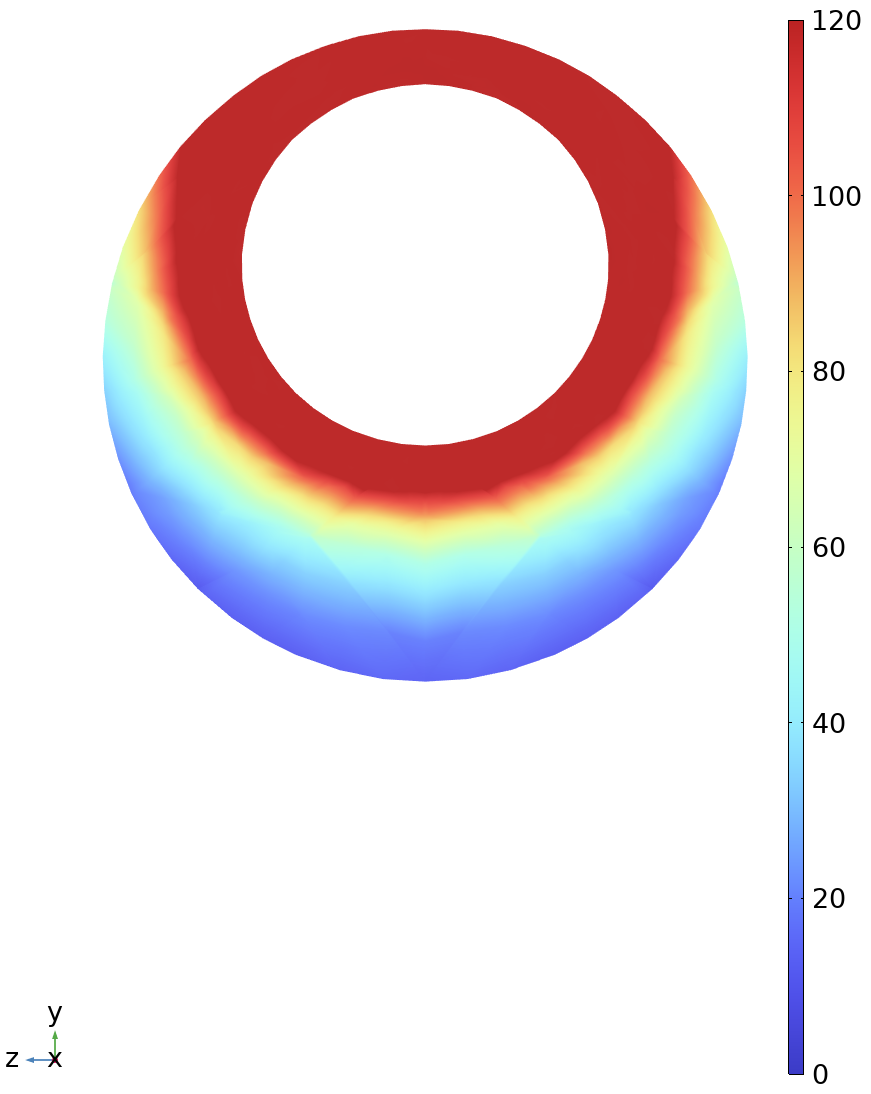
\includegraphics[width=\textwidth]{comsol_sc_bare_section_P90.png}
\caption{bare}
\end{subfigure}\qquad
\begin{subfigure}[b]{0.38\textwidth}\centering
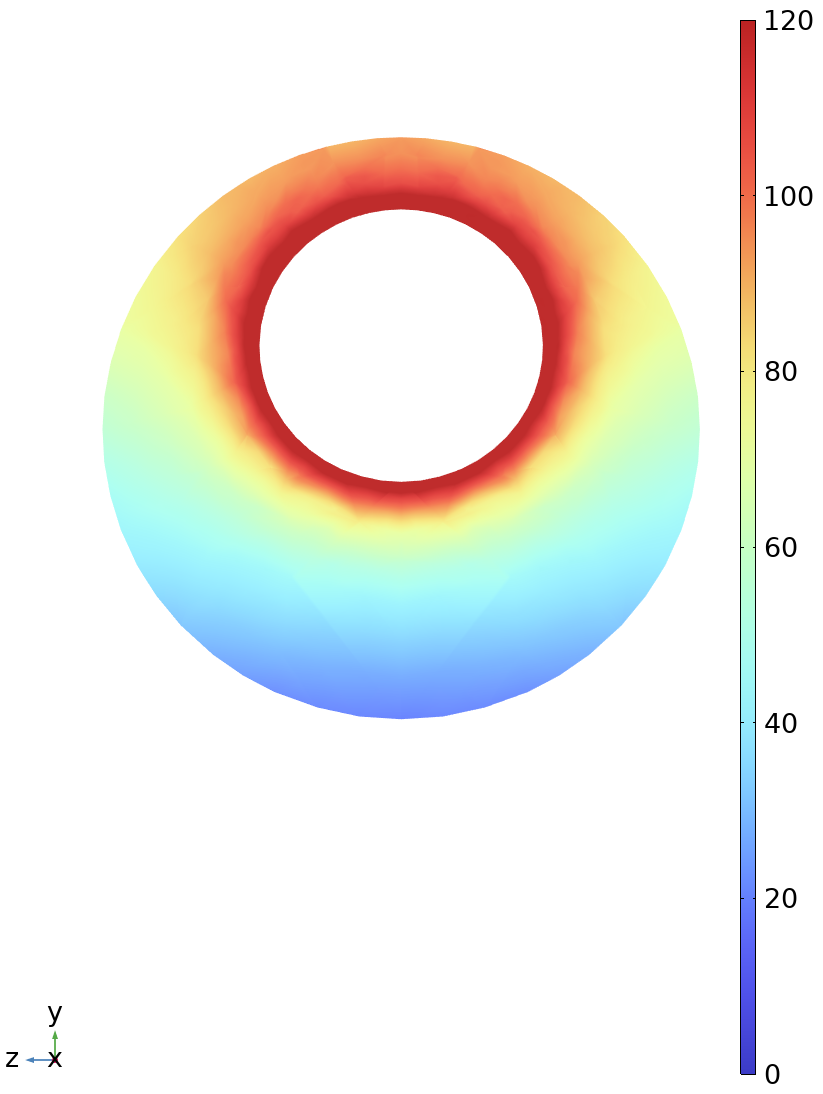
\includegraphics[width=\textwidth]{comsol_sc_sleeved_section_P90.png}
\caption{sleeved}
\end{subfigure}
\caption[Single-cavity actuator: section at mid-length (COMSOL)]{Single-cavity actuator at $P=\SI{90}{kPa}$: deformed section at $x=\SI{50}{mm}$, viewed along the
axis from the tip (COMSOL, true scale). Colour: von Mises stress [kPa], same scale in both panels; values
above \SI{120}{kPa} are shown in the top colour. Undeformed, the section is a circle of radius \SI{10}{mm}
with a cavity of radius \SI{4}{mm} centred \SI{3}{mm} above the axis.}
\label{fig:scsection}
\end{figure}

\section{Four-chamber actuator}\label{sec:res3}

\subsection{Bare and sleeved actuator}\label{sec:4chres}
Table~\ref{tab:4ch} and Figures~\ref{fig:4chresp}--\ref{fig:4chsection} give the results of the four-chamber
model of Chapter~\ref{ch:method} ($E=\SI{0.07}{MPa}$, $\mu=E/(2(1+\nu))=\SI{23.3}{kPa}$).

\begin{table}[H]
\centering\small
\caption[Four-chamber actuator: tip rotation with real pressure]{Four-chamber actuator, chamber~1 pressurised, $E=\SI{0.07}{MPa}$: tip rotation $\theta$ [\si{\degree}].
``Sleeved'' has the original chambers; ``filleted'' adds \SI{0.6}{mm} fillets to the chamber corners (\SI{0.24}{mm}
at the tip); ``deeper'' has chambers \SIrange{5.0}{1.5}{mm} deep and \ang{70} wide. Beam: eq.~(\ref{eq:taper}).
-- : no converged solution.}
\label{tab:4ch}
\begin{tabular}{@{}rccccc@{}}
\toprule
$P$ [kPa] & bare & sleeved & sleeved, filleted & sleeved, deeper & beam (sleeved)\\
\midrule
2 & 0.73 & 6.06 & 4.83 & 8.33 & 5.74\\
4 & 3.06 & 13.7 & 11.2 & 19.5 & 11.5\\
6 & 7.89 & 22.8 & 19.1 & 34.0 & 17.2\\
8 & 17.2 & 33.8 & 28.7 & 55.3 & 22.9\\
10 & 36.6 & 47.1 & 40.6 & -- & 28.7\\
12.5 & -- & 68.0 & 59.4 & -- & 35.8\\
15 & -- & 95.3 & 84.6 & -- & 43.0\\
\midrule
last converged step & \SI{11.7}{kPa} & \SI{20}{kPa} & \SI{21}{kPa} & \SI{8.5}{kPa} & \\
\bottomrule
\end{tabular}
\end{table}

\begin{figure}[H]
\centering
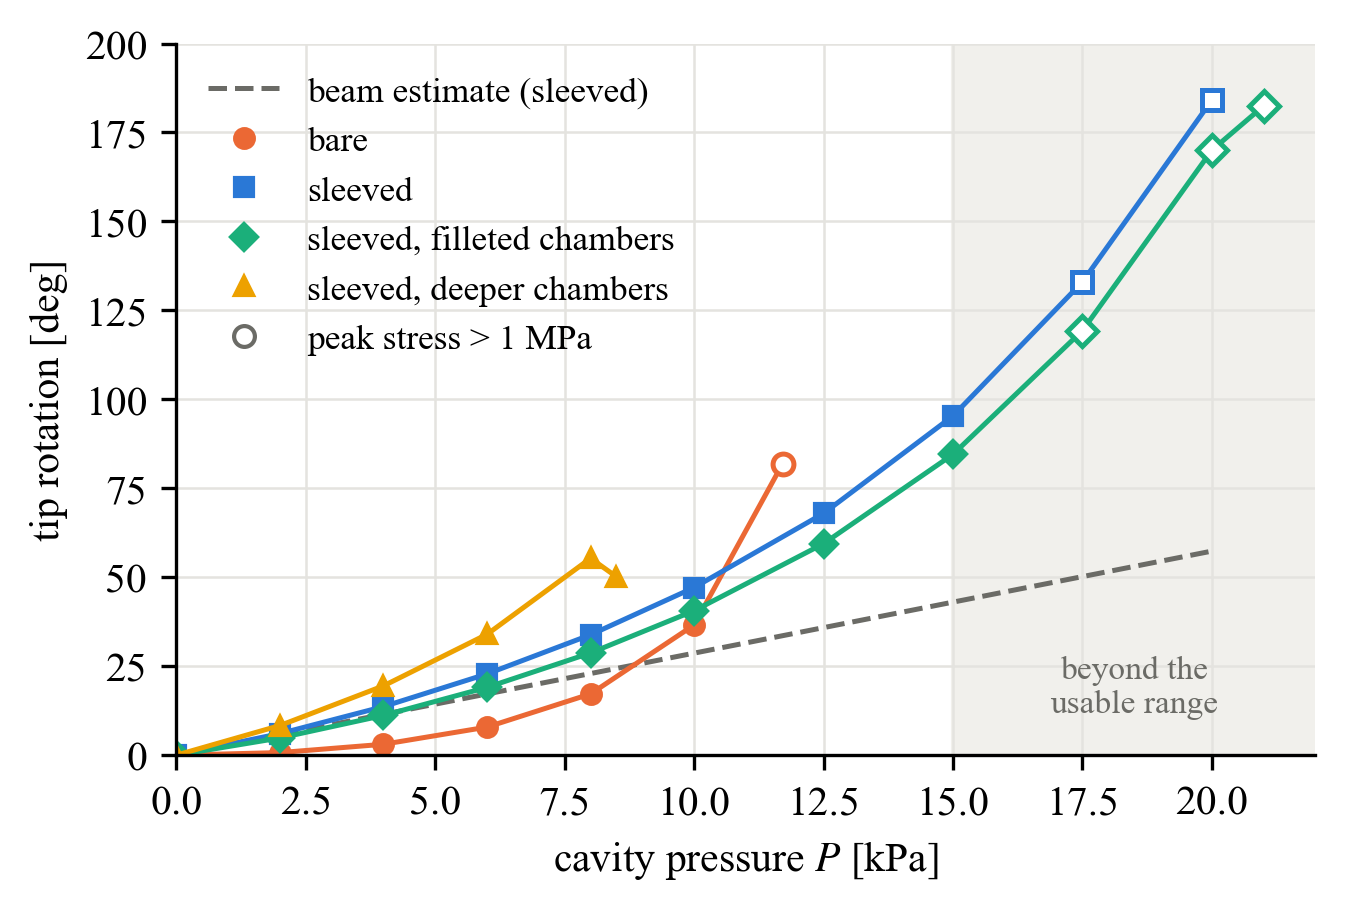
\includegraphics[width=0.72\textwidth]{fig_4ch_response.png}
\caption[Four-chamber actuator: tip rotation against pressure]{Four-chamber actuator with real pressure: tip rotation against pressure. Open symbols: steps where the
computed peak von Mises stress exceeds \SI{1}{MPa}. The shaded band lies beyond the range in which results are
used (Section~\ref{sec:limit}).}
\label{fig:4chresp}
\end{figure}

\begin{figure}[H]
\centering
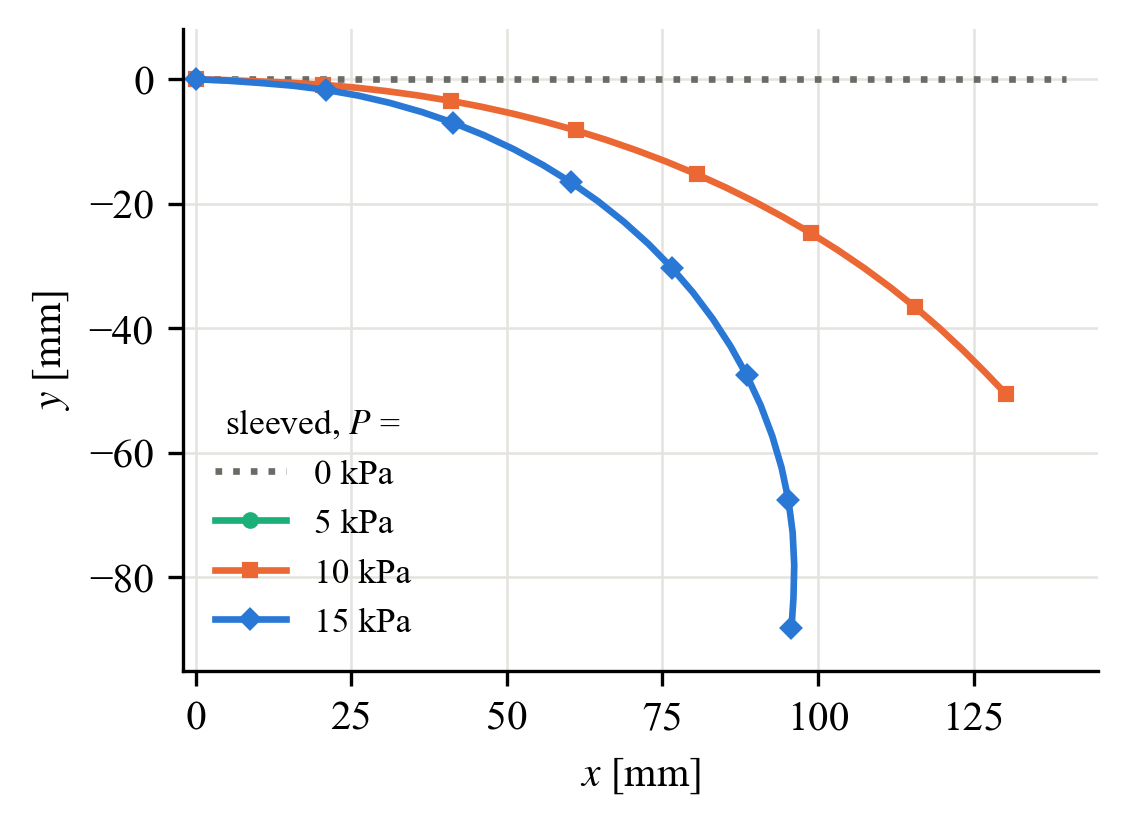
\includegraphics[width=0.72\textwidth]{fig_4ch_centreline.png}
\caption[Deformed centreline, sleeved four-chamber actuator]{Deformed centreline of the sleeved four-chamber actuator in the bending plane (true scale).}
\label{fig:centreline}
\end{figure}

\begin{figure}[H]
\centering
\begin{subfigure}[b]{0.49\textwidth}\centering
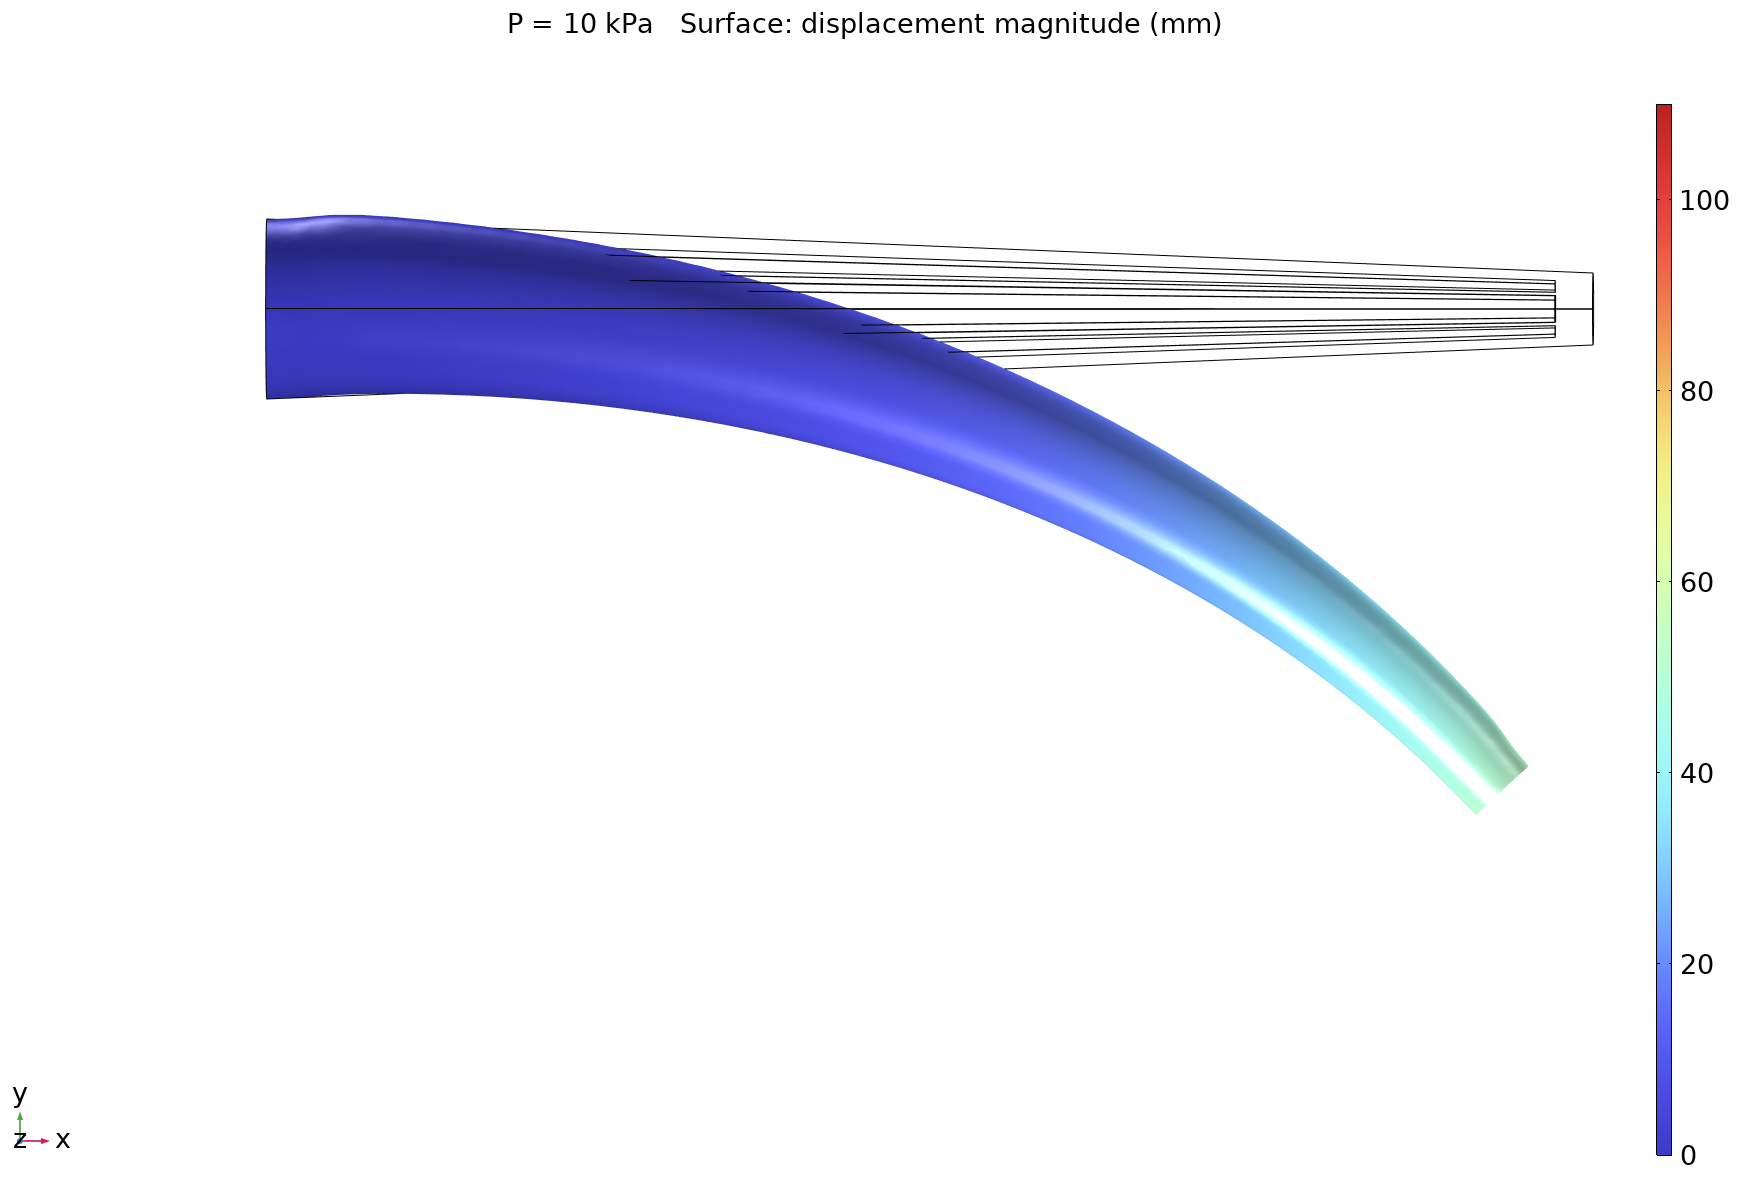
\includegraphics[width=\textwidth]{comsol_fc_sleeved_side_P10.png}
\caption{\SI{10}{kPa}, displacement [mm]}
\end{subfigure}\hfill
\begin{subfigure}[b]{0.49\textwidth}\centering
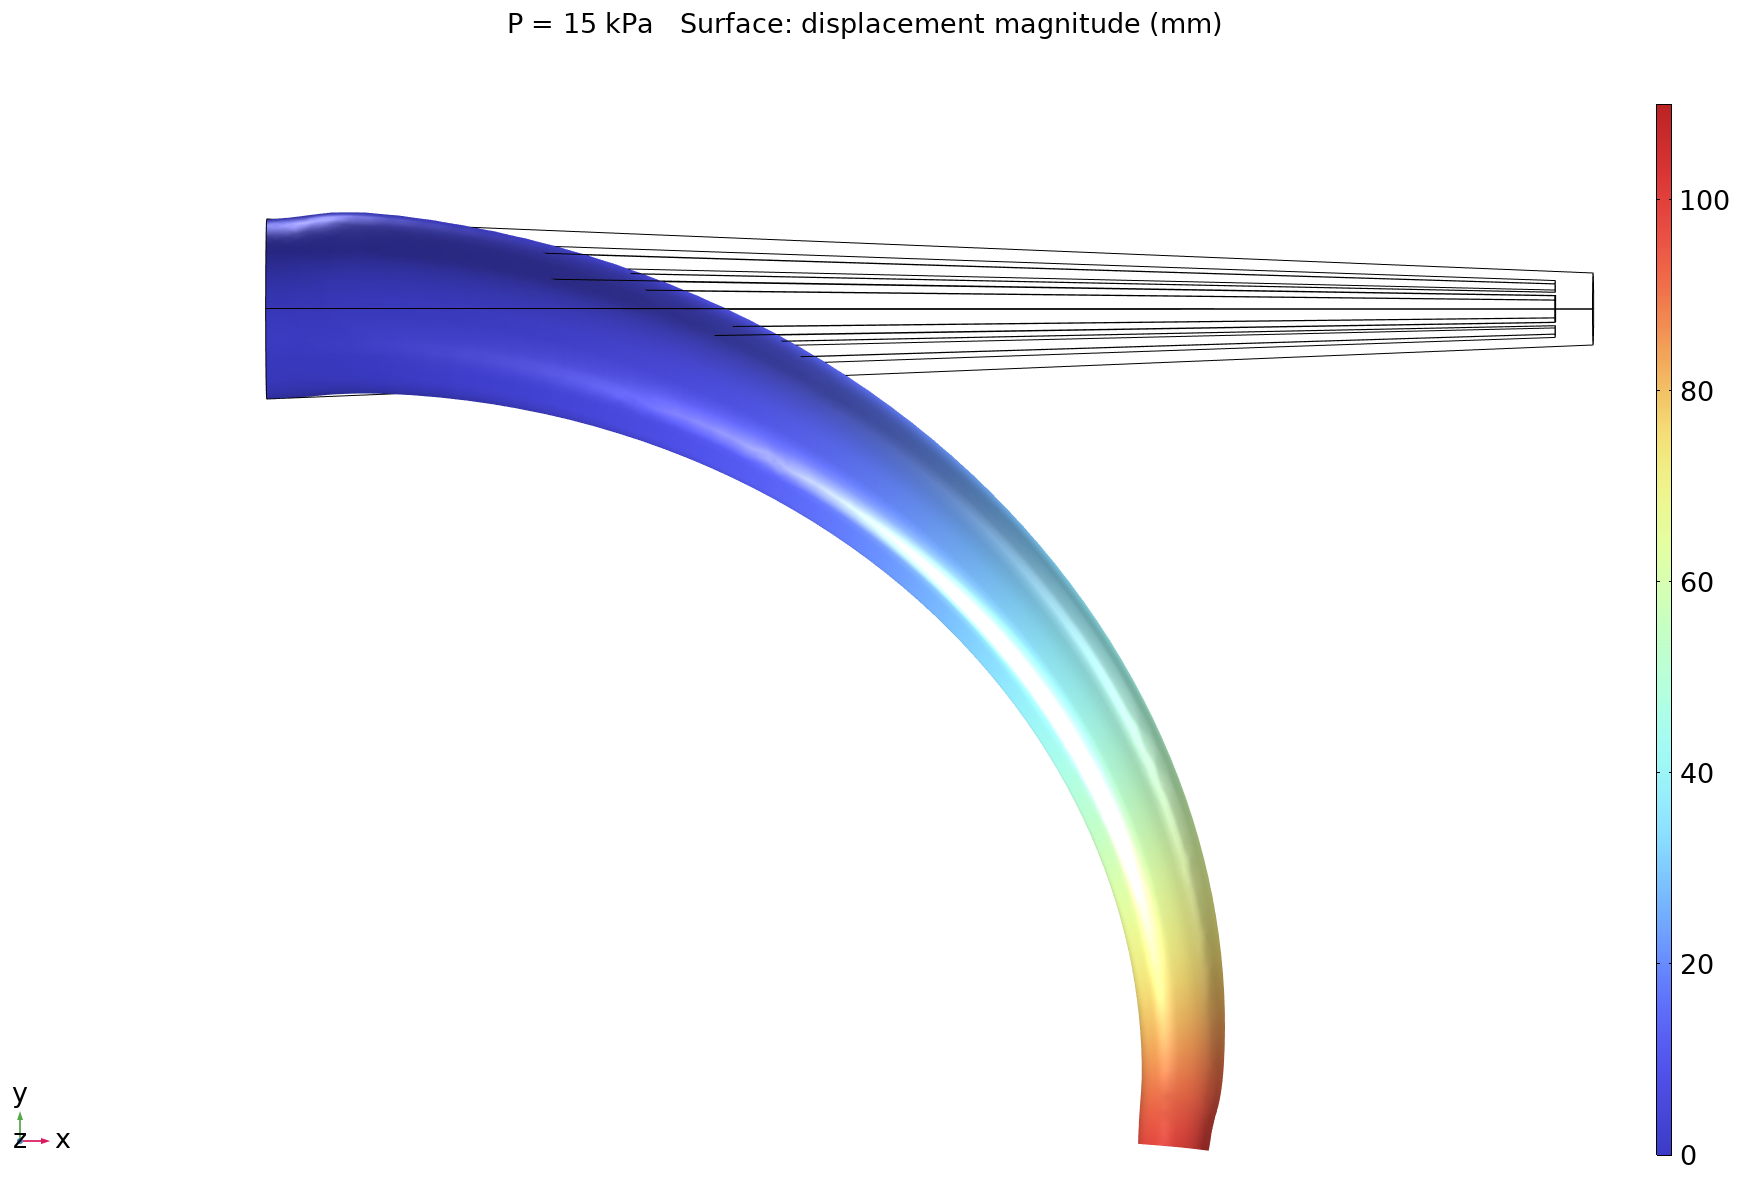
\includegraphics[width=\textwidth]{comsol_fc_sleeved_side_P15.png}
\caption{\SI{15}{kPa}, displacement [mm]}
\end{subfigure}

\vspace{4pt}
\begin{subfigure}[b]{0.55\textwidth}\centering
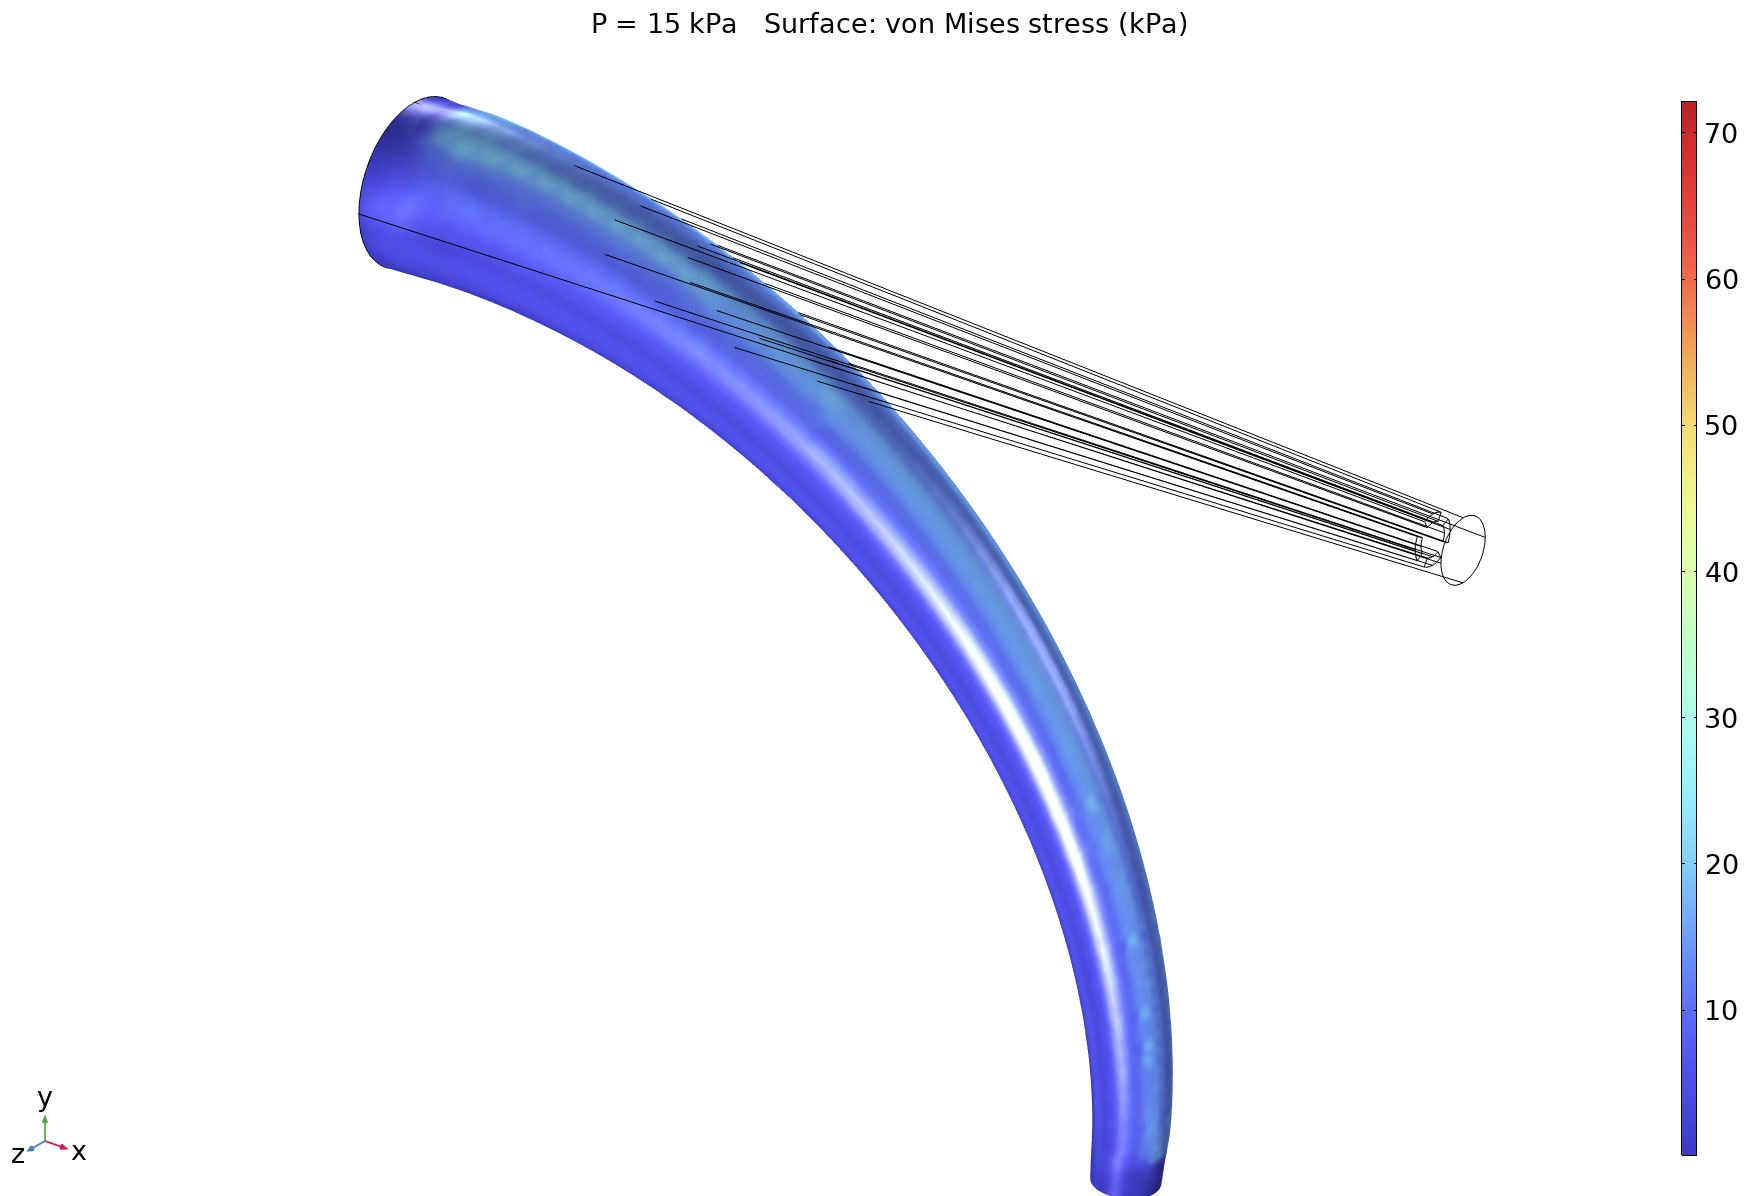
\includegraphics[width=\textwidth]{comsol_fc_sleeved_mises_P15.png}
\caption{\SI{15}{kPa}, von Mises stress on the outer surface [kPa], oblique view}
\end{subfigure}
\caption[Sleeved four-chamber actuator (COMSOL)]{Sleeved four-chamber actuator, $E=\SI{0.07}{MPa}$ (COMSOL, true scale; the thin lines show the
undeformed body). (a), (b) viewed normal to the bending plane, base clamped at the left. The colour scales
differ between panels; quantitative values are in Table~\ref{tab:4ch} and Figure~\ref{fig:centreline}. In
(c) only the outer surface is shown; the highest stresses lie inside the walls, at the chamber corners
(Section~\ref{sec:limit}).}
\label{fig:render}
\end{figure}

\begin{figure}[H]
\centering
\begin{subfigure}[b]{0.32\textwidth}\centering
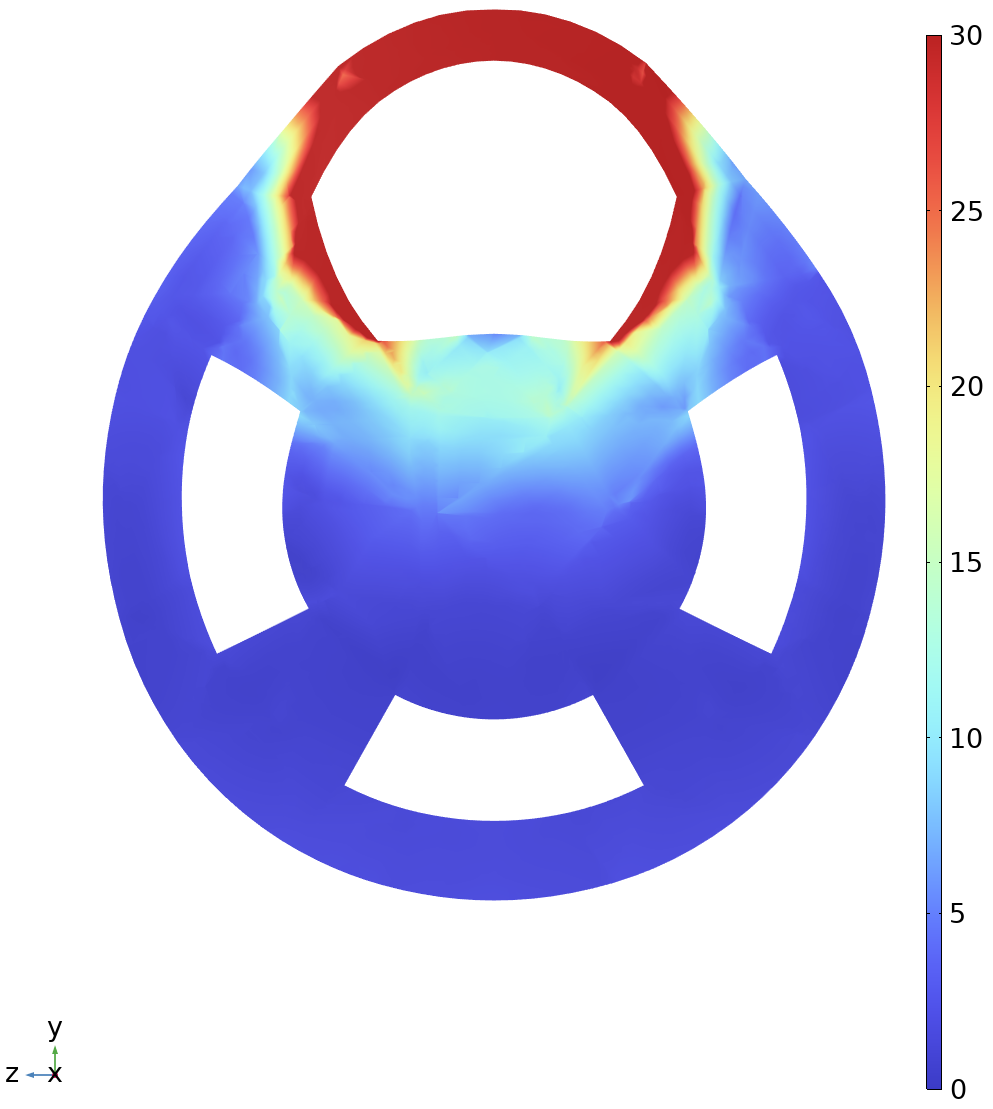
\includegraphics[width=\textwidth]{comsol_fc_bare_section_P10_x40.png}
\caption{bare}
\end{subfigure}\hfill
\begin{subfigure}[b]{0.32\textwidth}\centering
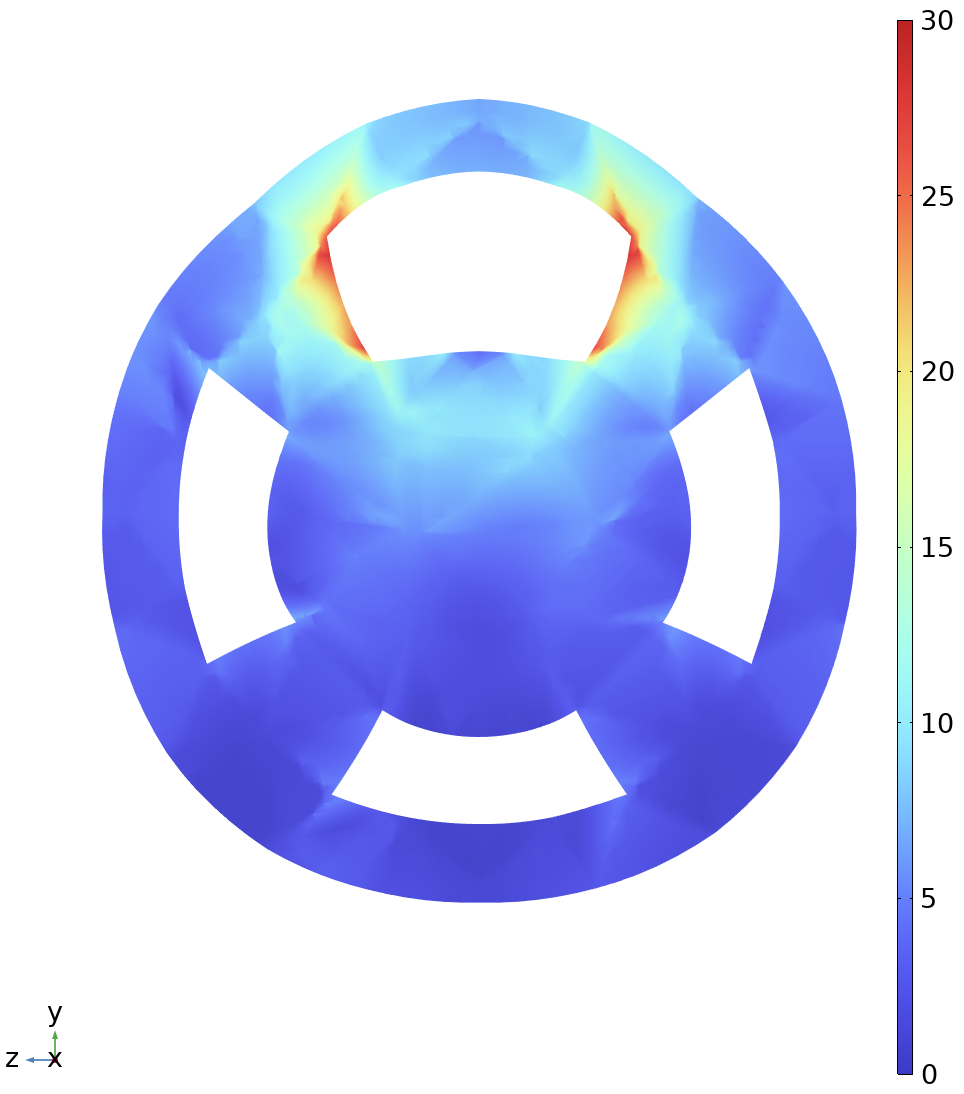
\includegraphics[width=\textwidth]{comsol_fc_sleeved_section_P10_x40.png}
\caption{sleeved}
\end{subfigure}\hfill
\begin{subfigure}[b]{0.32\textwidth}\centering
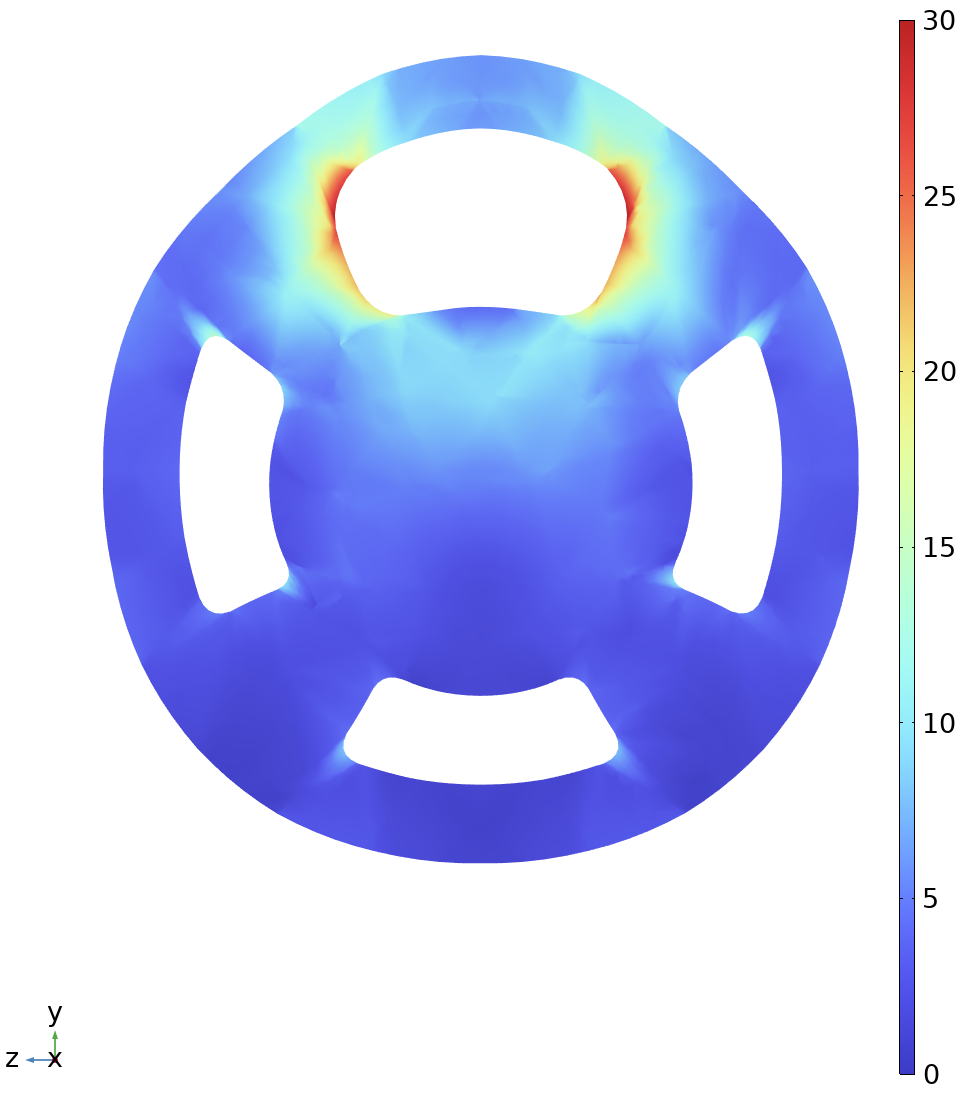
\includegraphics[width=\textwidth]{comsol_fc_fillet_section_P10_x40.png}
\caption{sleeved, filleted}
\end{subfigure}
\caption[Four-chamber actuator: section at 10 kPa (COMSOL)]{Four-chamber actuator at $P=\SI{10}{kPa}$: deformed section at $x=\SI{40}{mm}$, viewed along the axis
from the tip (COMSOL, true scale; chamber~1 at the top is pressurised). Colour: von Mises stress [kPa], same
scale in all three panels; values above \SI{30}{kPa} are shown in the top colour. Compare the undeformed
sections in Figure~\ref{fig:comsolsec}.}
\label{fig:4chsection}
\end{figure}

\paragraph{Bare.} The bare actuator bends little at first (\ang{0.73} at \SI{2}{kPa}) and then increasingly
fast, as the bare single-cavity actuator does. The section at mid-length grows by 13.8\,\% at \SI{10}{kPa},
and the solver stops at \SI{11.7}{kPa}, i.e.\ $P/\mu=0.50$, which is consistent with the onset of ballooning
of the chamber roof (Section~\ref{sec:wall}); the limit pressure was not located precisely. The last step is
not used: its computed stress is unphysical. Figure~\ref{fig:4chsection}(a) shows the section at
\SI{10}{kPa}: the roof of chamber~1 has bulged far beyond the original outer surface, and the stress is
highest in the roof and in the two ribs next to it.

\paragraph{Sleeved.} With the hoop sleeve the response starts linearly and close to the beam estimate
(\ang{6.06} against \ang{5.74} at \SI{2}{kPa}) and then bends more than the estimate, as the single-cavity
sleeved actuator does: \ang{47.1} at \SI{10}{kPa} and \ang{95.3} at \SI{15}{kPa}. The section at mid-length grows
by only 4.6\,\% at \SI{15}{kPa}. In the section of Figure~\ref{fig:4chsection}(b) the roof of chamber~1 stays
close to the original outer circle; the chamber widens, and the stress concentrates at its corners, where the
roof meets the ribs.

\paragraph{Chamber geometry.} Fillets on the chamber corners add material and reduce the bending by about
10\,\% (\ang{84.6} at \SI{15}{kPa}); at \SI{10}{kPa} the deformed section and its stress pattern are similar to those without
fillets (Figure~\ref{fig:4chsection}(c)). Deeper and wider chambers bend more at low pressure (\ang{55.3} at
\SI{8}{kPa}) but the rotation then decreases and the mid-length section shrinks: the thin ribs and the thin
core (radius \SIrange{2.5}{1.5}{mm}) collapse, and the solution stops at \SI{8.5}{kPa}. The beam estimate,
which assumes the section keeps its shape, had predicted that deeper chambers would be better; the FE result
shows that they are not.

\subsection{Range of the results}\label{sec:limit}
Above \SI{15}{kPa} the sleeved models still converge (to \SI{20}{kPa}, and \SI{21}{kPa} with fillets) and the
centreline continues to curl (to about \ang{180}), but two quantities grow rapidly:
\begin{itemize}
\item the computed peak von Mises stress, located at the junction between the roof of the pressurised
chamber and its side walls: in the sharp-cornered model \SI{0.25}{MPa} at \SI{15}{kPa}, \SI{1.04}{MPa} at
\SI{17.5}{kPa} and \SI{53}{MPa} at \SI{20}{kPa};
\item the local element distortion: the smallest local volume ratio $J$ falls from 0.92 at \SI{2}{kPa} to 0.30
at \SI{15}{kPa} and 0.01 at \SI{20}{kPa}, while the volume average of $J$ stays at 1.0000.
\end{itemize}
Fillets do not remove the stress growth, so it is not a sharp-corner singularity. Whether it is a physical
instability of the chamber wall junction or a numerical breakdown of the elements cannot be decided from these
runs. Results are therefore used only up to \SI{15}{kPa}; of these, only the \SI{10}{kPa} point has been
mesh-checked. For comparison, the tensile strength of Ecoflex 00-30 is about \SI{1.4}{MPa} \cite{ecoflex}.

\paragraph{Bending to \ang{180}: beyond the safe limit of the material.} Figure~\ref{fig:180} shows the sleeved
actuator at its last converged step, $P=\SI{20}{kPa}$, where the tip has rotated by \ang{184} and the actuator
has curled into a hook. This shape lies \emph{beyond the safe limit of the material}. At this step the computed
peak von Mises stress is \SI{53}{MPa}, about 38 times the tensile strength of Ecoflex 00-30 (about
\SI{1.4}{MPa} \cite{ecoflex}), the silicone whose stiffness is assumed in this model; already at
\SI{17.5}{kPa} (\ang{133}) the peak, \SI{1.04}{MPa}, is close to that strength. On the outer surface the stress stays well below
\SI{1.4}{MPa} (Figure~\ref{fig:180}(b)); the material above \SI{1.4}{MPa} is a small volume inside the
actuator, near the base end of chamber~1 (Figure~\ref{fig:180}(c), (d)). Whether this local stress is physical
or a numerical artefact is not resolved (see above), but as computed it exceeds the strength of the silicone,
so the material would be expected to fail there before the actuator reached \ang{180}. These figures therefore show what the model does, not a usable operating point; all
results quoted elsewhere in this report are for $P\le\SI{15}{kPa}$.

\begin{figure}[htbp]
\centering
\begin{subfigure}[b]{0.49\textwidth}\centering
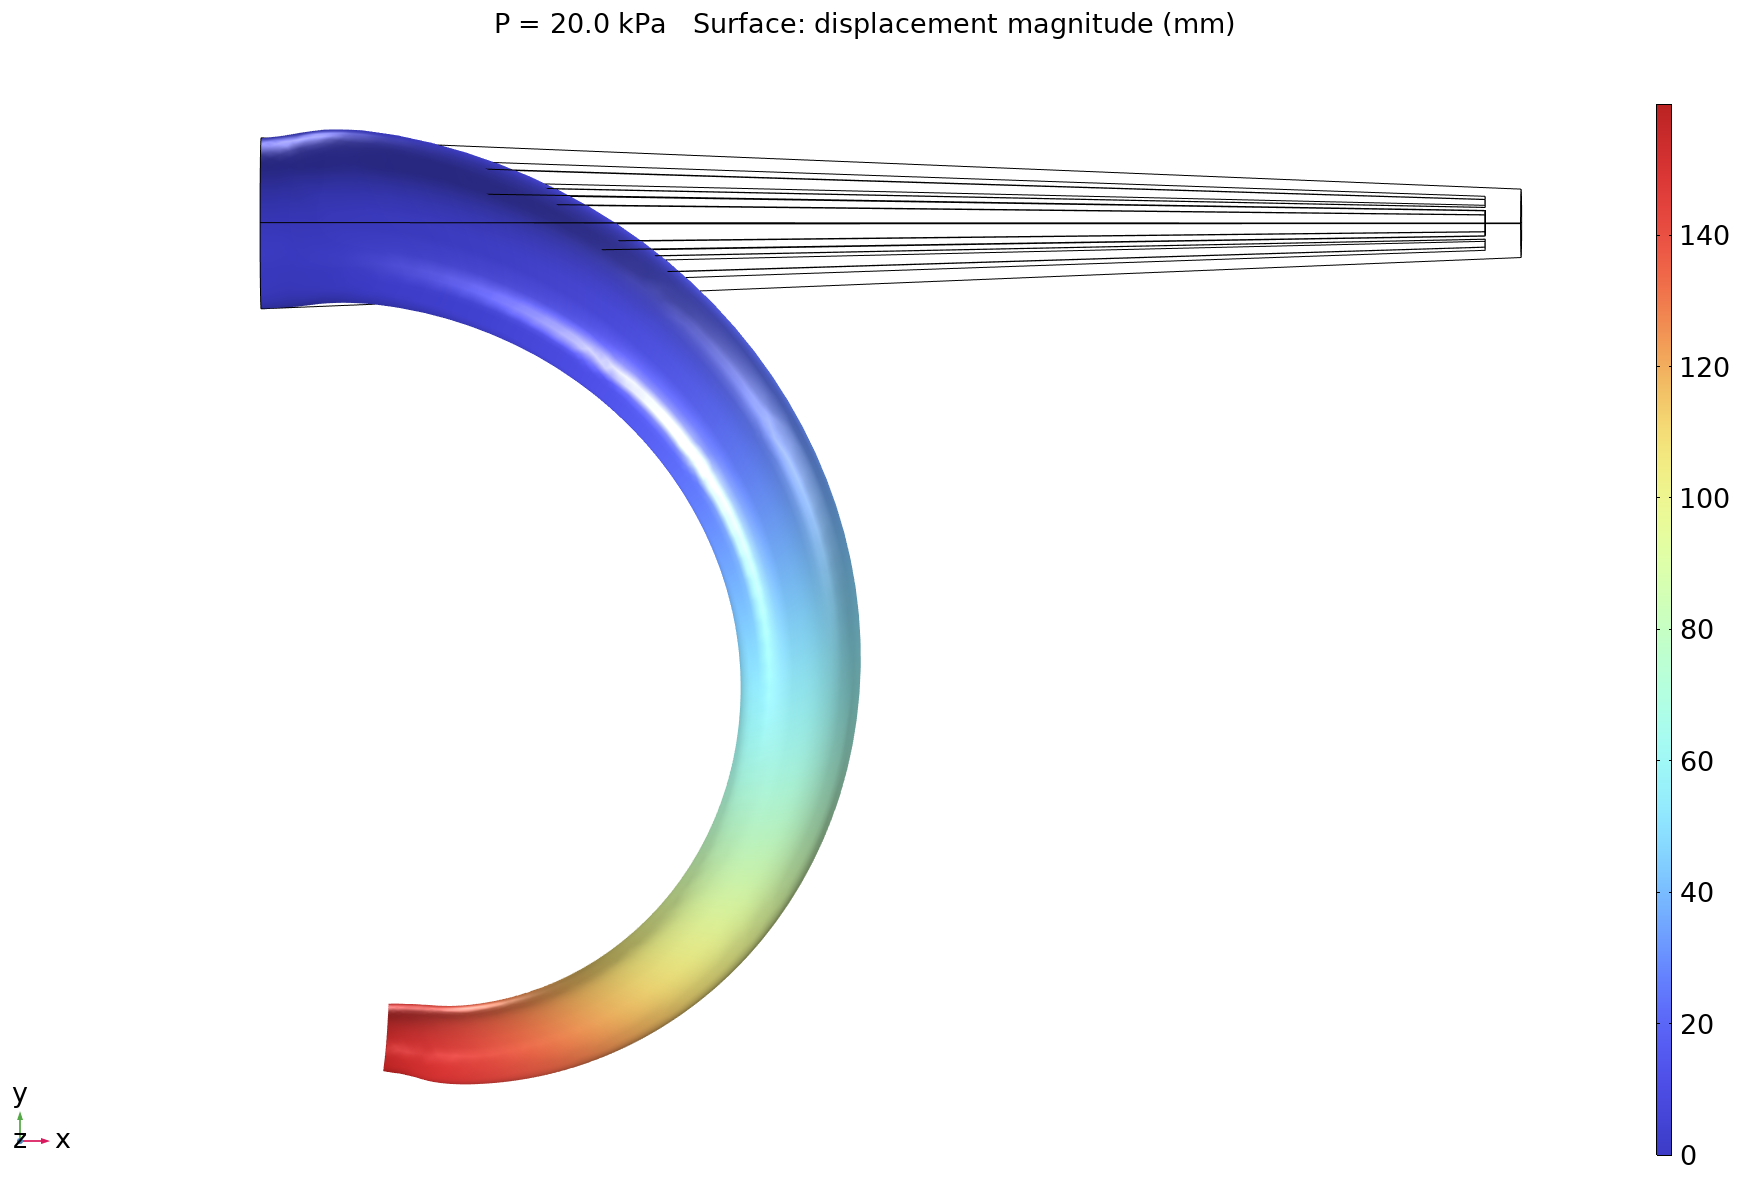
\includegraphics[width=\textwidth]{comsol_fc_sleeved_side_P20.png}
\caption{displacement magnitude [mm]}
\end{subfigure}\hfill
\begin{subfigure}[b]{0.49\textwidth}\centering
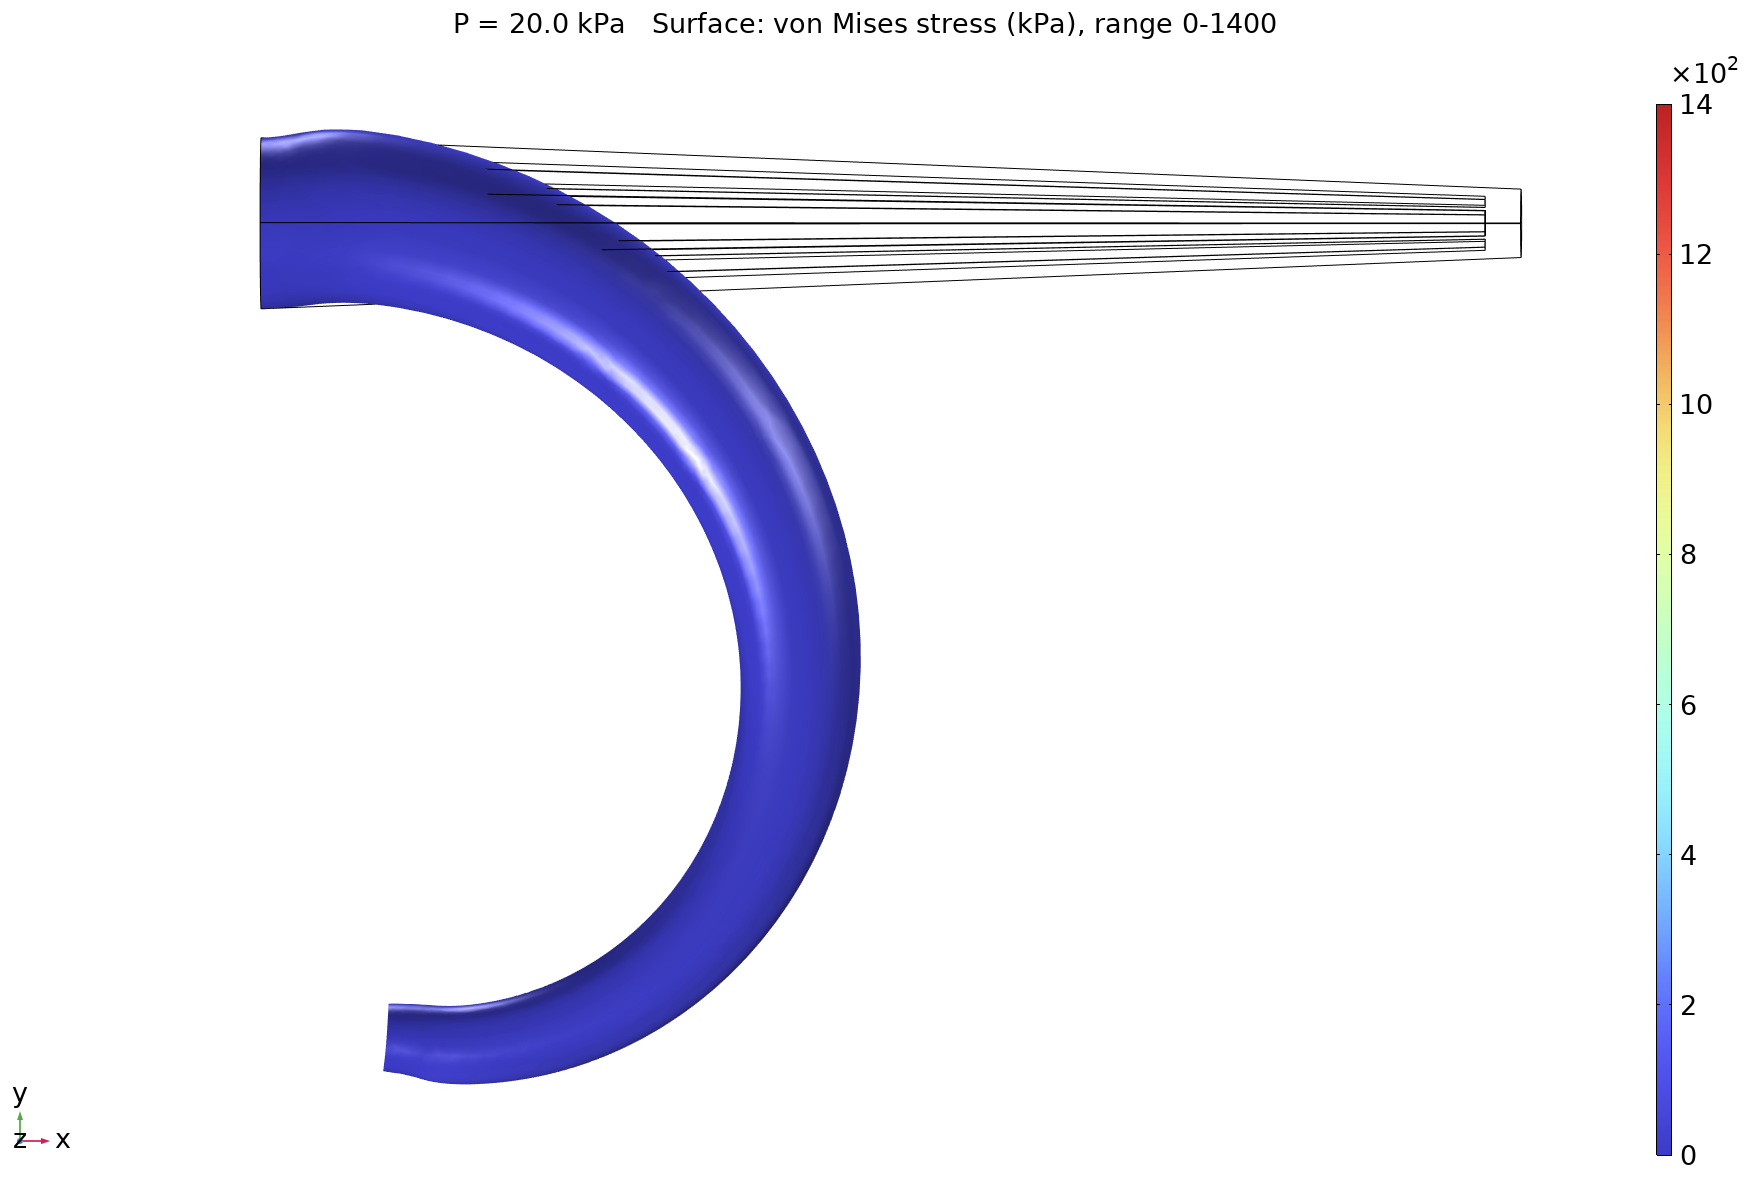
\includegraphics[width=\textwidth]{comsol_fc_sleeved_mises_side_P20.png}
\caption{von Mises stress on the outer surface [kPa], scale \SIrange{0}{1400}{kPa}}
\end{subfigure}

\vspace{4pt}
\begin{subfigure}[b]{0.49\textwidth}\centering
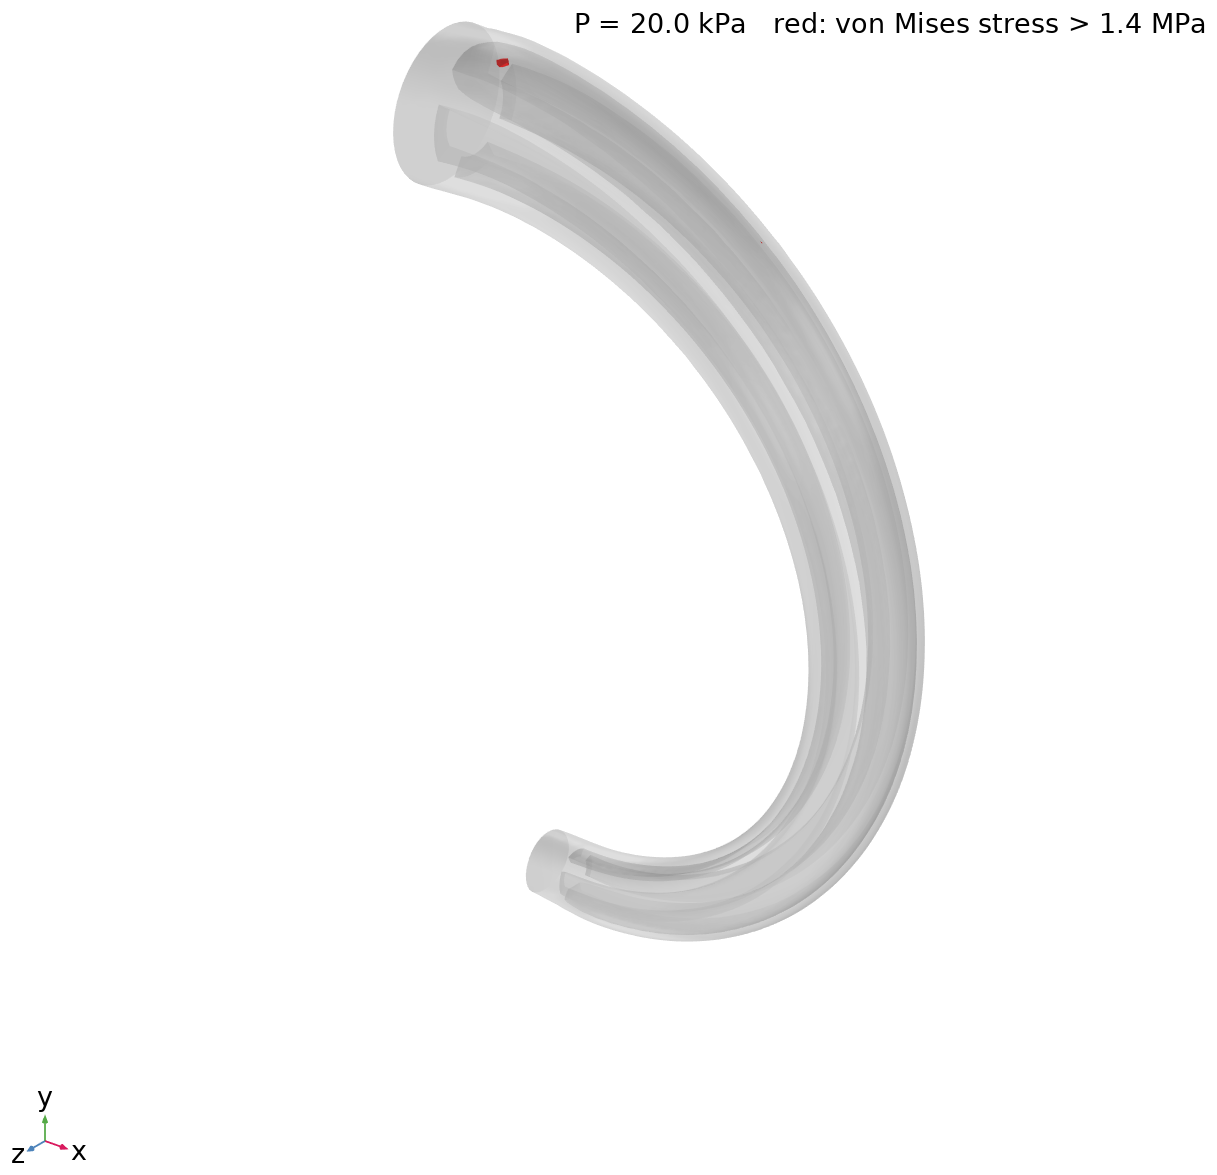
\includegraphics[width=\textwidth]{comsol_fc_sleeved_over_iso_P20.png}
\caption{oblique view; red: von Mises stress $>\SI{1.4}{MPa}$}
\end{subfigure}\hfill
\begin{subfigure}[b]{0.49\textwidth}\centering
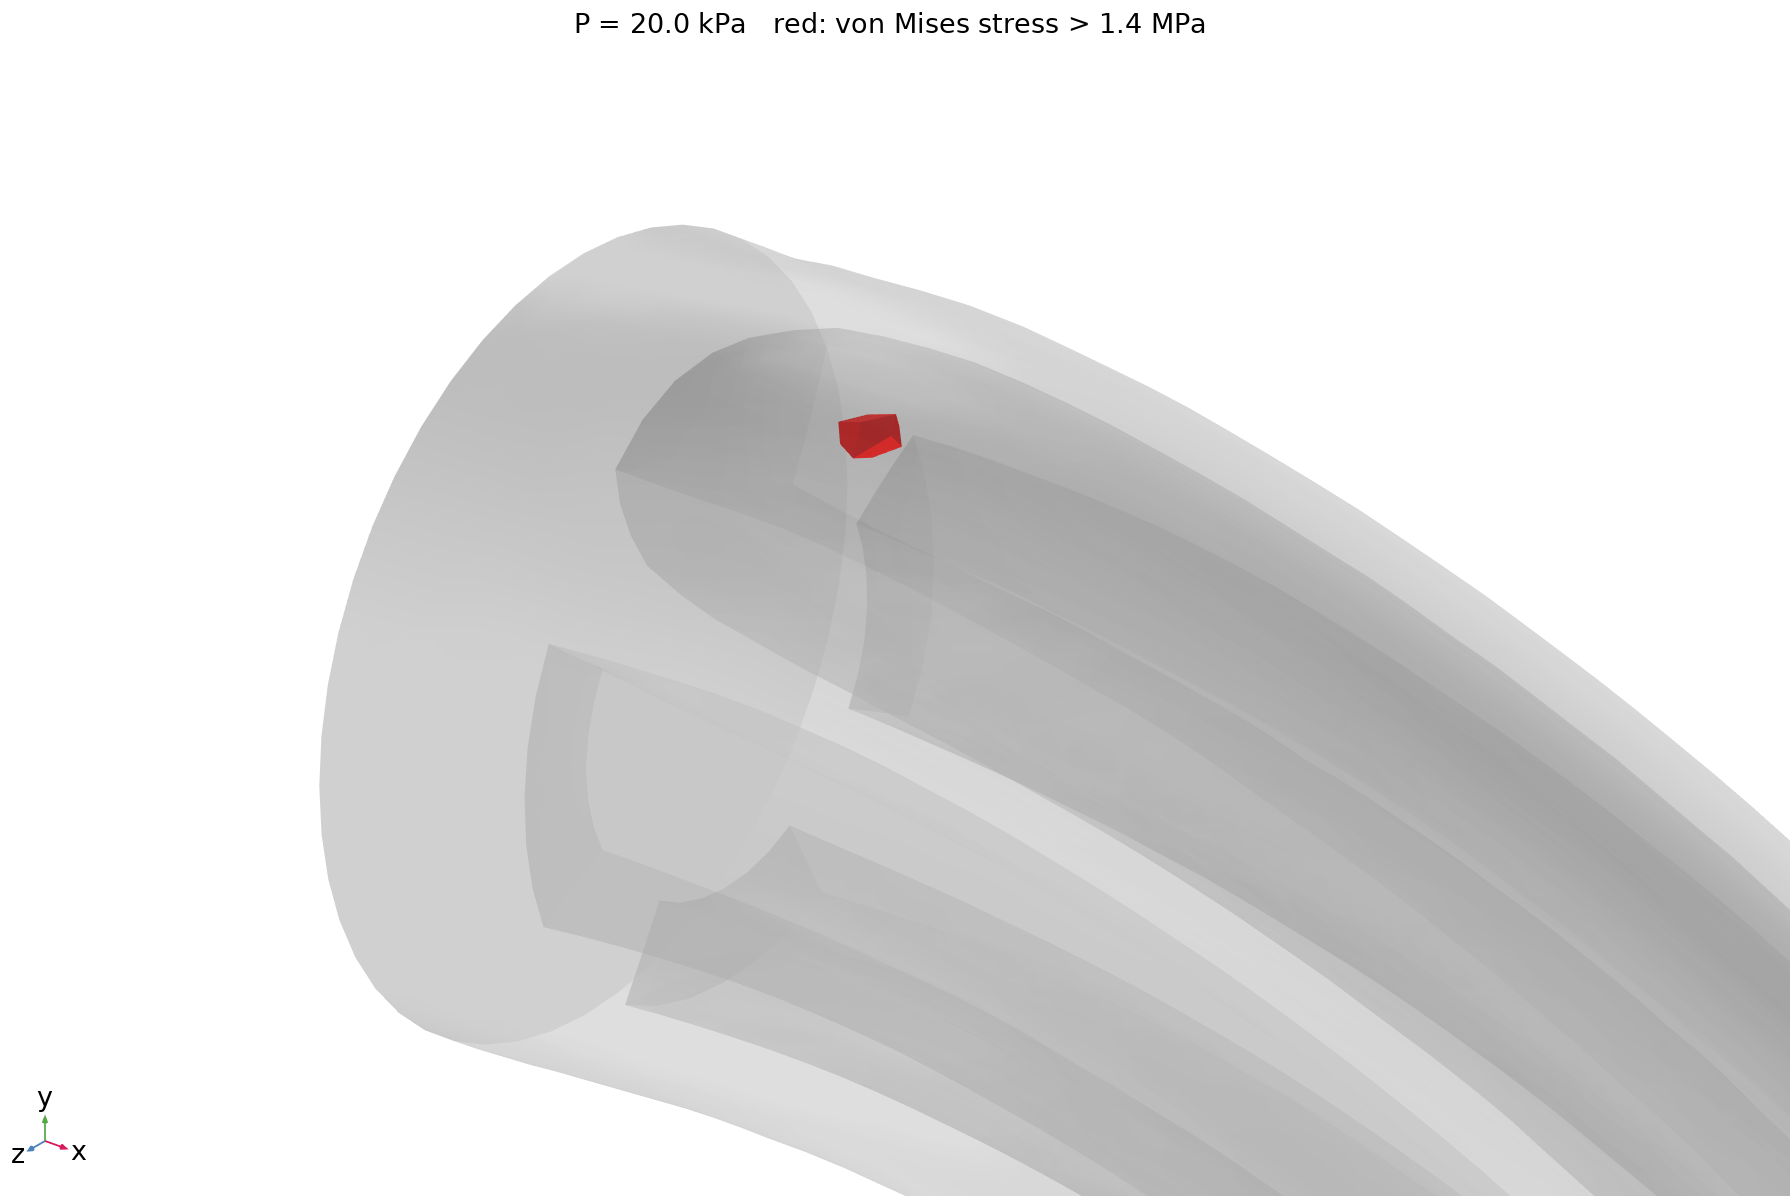
\includegraphics[width=\textwidth]{comsol_fc_sleeved_over_zoom_P20.png}
\caption{close-up of the base end of (c)}
\end{subfigure}
\caption[Sleeved four-chamber actuator at 20 kPa, tip rotation 184° (COMSOL)]{Sleeved four-chamber actuator, $E=\SI{0.07}{MPa}$, at $P=\SI{20}{kPa}$, the last converged step
(tip rotation \ang{184}; COMSOL, true scale; the thin lines in (a), (b) show the undeformed body; base clamped
at the left). In (c) and (d) the body is drawn transparent and the elements whose von Mises stress exceeds
\SI{1.4}{MPa}, the tensile strength of Ecoflex 00-30 \cite{ecoflex}, are shown in red. The computed peak is
\SI{53}{MPa}. \textbf{This state is beyond the safe limit of the material} and beyond the range in which the
results are used (Section~\ref{sec:limit}).}
\label{fig:180}
\end{figure}

% =====================================================================
\chapter{Discussion}\label{ch:discussion}
% =====================================================================

\section{How the actuator bends}
The analysis separates two mechanisms that the simple beam picture combines. The eccentric thrust moment,
eq.~(\ref{eq:M}), is always present and uniform, but in a bare incompressible actuator its effect is cancelled
at first order by the in-plane wall stresses, eq.~(\ref{eq:poisson}). What remains is the second-order
lengthening of the thin wall, eq.~(\ref{eq:twothirds}), which starts quadratically and ends at a ballooning
limit. A bare actuator is therefore weak at low pressure and unstable near the limit. The COMSOL model of the
single-cavity actuator shows this weak, steepening response; the limit pressure itself was not computed. With
a hoop reinforcement the in-plane cancellation is removed, the beam formula becomes the correct first-order
model, and the response is smooth up to the highest pressure simulated. The same picture holds for the tapered four-chamber actuator: bare, it balloons at
$P/\mu\approx0.5$; sleeved, it bends smoothly and starts close to the beam estimate.

\section{Choice of material}
For a neo-Hookean material the response depends on $P/\mu$ only. A softer silicone therefore gives the same
curve at a proportionally lower pressure, and a stiffer silicone at a higher pressure; the material alone
does not change how far a given geometry can bend. Any ballooning limit of a bare actuator, and the bending
reached before the stress growth of Section~\ref{sec:limit}, are fixed fractions of $\mu$ for a given geometry.
A real silicone stiffens at large stretch, which a Yeoh fit to measured data would capture; this may raise the
ballooning limit and delay the stress growth, and needs to be checked with the measured material.

\section{Checks on the FE models}
No second FE code and no experiment were available, so the FE results rest on the following checks:
\begin{itemize}
\item at small pressure the sleeved single-cavity model agrees with the closed-form beam result within 1\,\%
(\SI{10}{kPa}), which tests the geometry, the material constants, the follower load and the measurement of the
tip angle together;
\item the bare single-cavity model shows the large reduction of bending predicted by eq.~(\ref{eq:poisson});
\item the sleeved four-chamber model agrees with the tapered beam estimate, eq.~(\ref{eq:taper}), within 6\,\%
at \SI{2}{kPa};
\item the four-chamber tip rotation changes by 1.2\,\% with a finer mesh at \SI{10}{kPa};
\item the boundary classification of the four-chamber model is printed and checked for every run, so that the
pressure is known to act on the faces of chamber~1 only.
\end{itemize}
Every FE result in this report uses the real cavity pressure, applied uniformly to every face of the
pressurised cavity, and nearly incompressible silicone, so that the pressure axis of every figure is a
physical pressure that can be set in an experiment. What these checks do not cover is listed in
Section~\ref{sec:limits}.

\section{Towards grasping}\label{sec:grasp}
The long-term aim is a finger that curls around an object. With the present four-chamber geometry and a hoop
sleeve, about \ang{85}--\ang{95} of tip rotation is obtained within the range of trusted results, which is
less than needed to wrap an object. Contact with an object has not been simulated with the physical model,
so no grasping force is reported. To get there, the following are needed: resolving the stress growth of
Section~\ref{sec:limit} (finer local mesh or hexahedral wall elements), possibly thicker chamber side walls or a
longer actuator, measured material constants, and contact modelling with a stiff penalty or an augmented
Lagrangian formulation, with the wrap measured as the arc actually in contact.

\section{Limitations}\label{sec:limits}
\begin{itemize}
\item All dimensions and moduli are placeholders; $E=\SI{0.07}{MPa}$ for the four-chamber actuator is assumed.
\item Neo-Hookean material; strain stiffening, viscoelasticity and the Mullins effect are not modelled.
\item The sleeve is ideal: inextensible in hoop, no axial stiffness, perfectly bonded.
\item Only pitch bending (one chamber) of the four-chamber actuator has been computed with real pressure.
\item The four-chamber mesh check covers \SI{10}{kPa} only; the single-cavity models were not mesh-checked.
\item The FE models were not compared with a second FE code.
\item No experiment has been done, so no result is validated against a physical actuator.
\end{itemize}

% =====================================================================
\chapter{Conclusions and Future Work}\label{ch:conclusion}
% =====================================================================
\section{Conclusions}
\begin{enumerate}
\item The cross-section properties and the eccentric thrust moment of the actuator follow from statics; the
moment $M=\pi PR^2r^2\rp/(R^2-r^2)$ is uniform along the actuator for any material law.
\item The Euler--Bernoulli result, eq.~(\ref{eq:theta}), is the correct first-order model of a
\emph{hoop-reinforced} actuator: the COMSOL tip angle agrees with it within 1\,\% at $P/E=0.017$ and 5\,\% at
$P/E=0.033$, and exceeds it at higher pressure.
\item For a \emph{bare} silicone actuator the first-order bending vanishes by the factor $(1-2\nu)$. The bending
that remains comes from second-order wall lengthening and is limited by ballooning. In COMSOL the bare
actuator bends only 11\,\% of the beam value at $P/E=0.017$, and its response steepens strongly with pressure.
\item Parametric, scripted COMSOL models with a follower cavity pressure, nearly incompressible neo-Hookean
silicone and a weak-form hoop sleeve were set up for both actuators and can be re-run for the real design.
\item A tapered four-chamber actuator with a hoop sleeve bends smoothly under real pressure, to about \ang{95} at
$P/\mu=0.64$ (\SI{15}{kPa} for $E=\SI{0.07}{MPa}$); without the sleeve it balloons at $P/\mu=0.50$. Deeper and
wider chambers collapse; fillets reduce the bending slightly. Larger angles are not yet reliable.
\end{enumerate}

\section{Future work}
\begin{enumerate}
\item Resolve the stress growth above $P/\mu\approx0.64$ in the four-chamber model (local mesh refinement or
hexahedral wall elements, then thicker side walls if it is physical).
\item Mesh-check the single-cavity models and continue the bare model to its ballooning limit (with a
volume-controlled or arc-length solution).
\item Fix the real geometry and silicone; measure the material (uniaxial tests, Yeoh fit) and re-run the models.
\item Compute yaw and combined bending of the four-chamber actuator with real pressure.
\item Model contact with objects with a stiff contact formulation, then grasping.
\item Fabricate the actuator (moulding and casting \cite{marchese2015}) and measure pressure, tip angle and cavity
volume to validate the models.
\end{enumerate}

% =====================================================================
%  REFERENCES
% =====================================================================
\renewcommand{\bibname}{References}
\begin{thebibliography}{99}
\bibitem{gorissen2017} B.~Gorissen, D.~Reynaerts, S.~Konishi, K.~Yoshida, J.-W.~Kim and M.~De~Volder,
``Elastic inflatable actuators for soft robotic applications,'' \emph{Advanced Materials}, vol.~29, no.~43,
p.~1604977, 2017. doi:10.1002/adma.201604977.
\bibitem{marchese2015} A.~D.~Marchese, R.~K.~Katzschmann and D.~Rus, ``A recipe for soft fluidic elastomer
robots,'' \emph{Soft Robotics}, vol.~2, no.~1, pp.~7--25, 2015. doi:10.1089/soro.2014.0022.
\bibitem{polygerinos2015} P.~Polygerinos, Z.~Wang, J.~T.~B.~Overvelde, K.~C.~Galloway, R.~J.~Wood, K.~Bertoldi
and C.~J.~Walsh, ``Modeling of soft fiber-reinforced bending actuators,'' \emph{IEEE Transactions on Robotics},
vol.~31, no.~3, pp.~778--789, 2015. doi:10.1109/TRO.2015.2428504.
\bibitem{connolly2017} F.~Connolly, C.~J.~Walsh and K.~Bertoldi, ``Automatic design of fiber-reinforced soft
actuators for trajectory matching,'' \emph{Proceedings of the National Academy of Sciences}, vol.~114, no.~1,
pp.~51--56, 2017. doi:10.1073/pnas.1615140114.
\bibitem{gere2013} J.~M.~Gere and B.~J.~Goodno, \emph{Mechanics of Materials}, 8th ed. Stamford, CT: Cengage
Learning, 2013.
\bibitem{timoshenko1970} S.~P.~Timoshenko and J.~N.~Goodier, \emph{Theory of Elasticity}, 3rd ed. New York:
McGraw-Hill, 1970.
\bibitem{treloar1975} L.~R.~G.~Treloar, \emph{The Physics of Rubber Elasticity}, 3rd ed. Oxford: Clarendon
Press, 1975.
\bibitem{holzapfel2000} G.~A.~Holzapfel, \emph{Nonlinear Solid Mechanics: A Continuum Approach for Engineering}.
Chichester: Wiley, 2000.
\bibitem{yeoh1993} O.~H.~Yeoh, ``Some forms of the strain energy function for rubber,'' \emph{Rubber Chemistry
and Technology}, vol.~66, no.~5, pp.~754--771, 1993. doi:10.5254/1.3538343.
\bibitem{webster2010} R.~J.~Webster~III and B.~A.~Jones, ``Design and kinematic modeling of constant curvature
continuum robots: a review,'' \emph{International Journal of Robotics Research}, vol.~29, no.~13,
pp.~1661--1683, 2010. doi:10.1177/0278364910368147.
\bibitem{gent2005} A.~N.~Gent, ``Elastic instabilities in rubber,'' \emph{International Journal of Non-Linear
Mechanics}, vol.~40, nos.~2--3, pp.~165--175, 2005. doi:10.1016/j.ijnonlinmec.2004.05.006.
\bibitem{comsol} COMSOL AB, \emph{COMSOL Multiphysics Reference Manual}, version~6.4. Stockholm, Sweden.
\bibitem{comsolsm} COMSOL AB, \emph{Structural Mechanics Module User's Guide}, version~6.4. Stockholm,
Sweden.
\bibitem{ecoflex} Smooth-On, Inc., \emph{Ecoflex Series Technical Bulletin} (Ecoflex 00-30: tensile strength
200~psi, 100\,\% modulus 10~psi, elongation at break 900\,\%).
\end{thebibliography}

% =====================================================================
%  APPENDIX
% =====================================================================
\appendix
\titleformat{\chapter}[display]{\normalfont\bfseries\centering}{\large APPENDIX \thechapter}{6pt}{\Large\MakeUppercase}
\chapter{Software, Data and Reproduction}\label{app:files}
The scripts, solved COMSOL models (\texttt{.mph} files), data files and the \LaTeX{} source of this report are
available in the project's GitHub repository:
\begin{center}
\url{https://github.com/ItzRnP-hardcore/modelling_soft_polymer_based_actuator}
\end{center}
The paths in Table~\ref{tab:files} are relative to the root of that repository.
\begin{table}[H]
\centering\small
\caption[Files behind the results]{Files behind the results of this report (paths relative to the root of the GitHub repository).}
\label{tab:files}
\begin{tabularx}{\textwidth}{@{}>{\raggedright\arraybackslash}p{7.2cm}>{\raggedright\arraybackslash}X@{}}
\toprule
File & Content\\
\midrule
\path{actuator_model.py} & beam model, Tiers 1--3\\
\path{comsol/bare/BuildActuatorBare.java} & bare single-cavity model; results in \path{comsol_bare_summary.csv} (Table~\ref{tab:fe})\\
\path{comsol/sleeved/BuildActuatorSleeve.java} & sleeved single-cavity model; results in \path{comsol_sleeve_summary.csv} (Table~\ref{tab:fe})\\
\path{comsol/tapered_4cavity_sleeved/BuildActuator4CavitySleeved.java} & four-chamber model (all cases)\\
\path{comsol/tapered_4cavity_sleeved/run_sleeved_study.py} & runs the four cases and writes \path{sleeved_study_summary.csv} and \path{sleeved_study_centreline.csv} (Table~\ref{tab:4ch})\\
\path{report/btp_report/make_report_figures.py} & figures of Chapter~\ref{ch:results} from the data files\\
\path{report/btp_report/render/RenderReport.java} & COMSOL images (Figures~\ref{fig:comsolsec}, \ref{fig:mesh}, \ref{fig:scside}, \ref{fig:scsection}, \ref{fig:render}, \ref{fig:4chsection}) from the solved \path{.mph} files; also re-evaluates the single-cavity tip angles as a check\\
\path{report/btp_report/render/crop_renders.py} & crops those images for the report\\
\path{report/btp_report/render/Render180.java}, \path{crop_180.py} & images of the \SI{20}{kPa} step (Figure~\ref{fig:180}) and its peak stresses\\
\bottomrule
\end{tabularx}
\end{table}

\noindent Commands (from the project folder):
\begin{small}
\begin{verbatim}
comsolcompile BuildActuatorSleeve.java        (in comsol/sleeved/)
comsolbatch -inputfile BuildActuatorSleeve.class
python comsol/tapered_4cavity_sleeved/run_sleeved_study.py
python report/btp_report/make_report_figures.py
comsolcompile RenderReport.java               (in report/btp_report/render/)
comsolbatch -inputfile RenderReport.class
python render/crop_renders.py                 (in report/btp_report/)
\end{verbatim}
\end{small}

\end{document}
